\section{Concentration for $c(k; \Gbox)$ (Proving Proposition \ref{prop:concentration_local_clustering_P_n})}
\label{sec:concentration_c_P_n}

In this section we establish a concentration result for the local clustering function $c^\ast(k; \Gbox)$ in the finite box model $\Gbox$. Similar to the previous section we will focus on typical points $p = (0,y)$ with $y \in \Kcal_{C}(k_n)$.

\subsection{The main contribution of triangles}

First we write
\[
	c^\ast(k_n ; \Gbox) = \frac{T_{\text{box}}(k_n)}{\binom{k_n}{2}\Exp{\Nbox(k_n)}},
\]
where
\[
	 T_{\text{box}}(k_n) = \sum_{p \in \Pcal} \ind{\Dbox(p) = k_n} \sum_{p_1, p_2 \in \Pcal \setminus p}^{\ne} 
	 \ind{p_1 \in \BallPon{p}}\ind{p_2 \in \BallPon{p}}\ind{p_2 \in \BallPon{p_1}}
\]
In particular, the variance of $c^\ast(k_n ; \Gbox)$ is determined by the variance of $T_{\text{box}}(k_n)$.

Next, recall the adjusted triangle count function
\[
	\widetilde{T}_{\text{box}}(p_0) = \sum_{(p_1, p_2) \in \Pcal \setminus p_0}^{\ne} 
		\widetilde{T}_{\text{box}}(p_0,p_1,p_2).
\]
where
\[
	\widetilde{T}_{\text{box}}(p_0,p_1,p_2) = \ind{p_1 \in \BallPon{p_0}}\ind{p_2 \in \BallPon{p_0}}\ind{p_2 \in \BallPo{p_1} \cap \Rcal},
\]
and recall the definition of $\Kcal_{C}(k_n)$
\[
	\Kcal_{C}(k_n) = \left\{y \in \R_+ : \frac{k_n - C \sqrt{k_n \log(k_n)}}{\xi} \vee 1 \le e^{\frac{y}{2}}
		\le \frac{k_n + C \sqrt{k_n \log(k_n)}}{\xi} \right\},
\]
and write $\Rcal(k_n,C) = [-I_n,I_n] \times \Kcal_{C}(k_n)$ for the part of the box $\Rcal$ with heights in $\Kcal_{C}(k_n)$.
Slightly abusing notation, we will define the corresponding triangle degree function
\begin{equation}\label{eq:def_degree_triangle_count_in_K}
	\widetilde{T}_{\text{box}}(k_n, C) = \sum_{p \in \Pcal \cap \Rcal(k_n,C)} \ind{\text{deg}_{\text{box}}(p) = k_n} \widetilde{T}_{\text{box}}(p).
\end{equation}
and with that a different clustering function.
\begin{equation}\label{eq:def_tilde_c_box}
	\widetilde{c}_{\text{box}}(k_n) = \frac{\widetilde{T}_{\text{box}}(k_n,C)}{\binom{k_n}{2}\Exp{N_{\text{box}}(k_n)}}
\end{equation}
The idea is that the main contribution of triangles of degree $k_n$ to the triangle count $T_{\text{box}}(k_n)$ is given by $\widetilde{T}_{\text{box}}(k_n, C)$. Therefore, in order to prove Proposition \ref{prop:concentration_local_clustering_P_n} it suffices to show that $\widetilde{T}_{\text{box}}(k_n,C)$ is sufficiently concentrated around its mean. This last part is done in the following proposition.

%\subsection{The proof of Proposition \ref{prop:concentration_local_clustering_P_n}}
%
%We start with the concentration result for $\widetilde{T}_{\text{box}}(k_n)$.

\begin{proposition}[Concentration $\widetilde{T}_{\text{box}}(k_n,C)$]\label{prop:concentration_tilde_T_P_n}
Let $\alpha > \frac{1}{2}$, $\nu > 0$ and let $(k_n)_{n \ge 1}$ be any positive sequence satisfying $k_n = \smallO{n^{\frac{1}{2\alpha+1}}}$. Then for any $C > 0$, as $n \to \infty$,
\[
	\Exp{\widetilde{T}_{\text{box}}(k_n,C)^2} = \left(1 + \smallO{1}\right)\Exp{\widetilde{T}_{\text{box}}(k_n, C)}^2.
\]
\end{proposition}

We first use this result to prove Proposition~\ref{prop:concentration_local_clustering_P_n}. The remainder of this section is devoted to prove Proposition~\ref{prop:concentration_tilde_T_P_n}. The final proof can be found in Section~\ref{ssec:concentration_tilde_T}.

\begin{proof}[Proof of Proposition \ref{prop:concentration_local_clustering_P_n}]
We bound the expectation as follows,
\begin{align*}
	\Exp{\left|c^\ast(k_n; \Gbox) - \Exp{c^\ast(k_n; \Gbox)}\right|} 
	&\le \frac{\Exp{\left|\widetilde{T}_{\text{box}}(k_n,C) - \Exp{\widetilde{T}_{\text{box}}(k_n,C)}\right|}}
		{\binom{k_n}{2}\Exp{N_{\text{box}}(k_n)}}\\
	&\hspace{10pt} + 2 \Exp{\left|c^\ast(k_n; \Gbox) - \widetilde{c}_{\text{box}}(k_n)\right|}.
\end{align*}
We will show that both terms are $\smallO{s(k_n)}$.

First we note that $\ind{p_2 \in \BallPo{p_1} \cap \Rcal} \le \ind{p_2 \in \BallPon{p_1}}$ and hence $\widetilde{T}_{\text{box}}(p) \le T_{\text{box}}(p)$. This implies that
\[
	 \widetilde{c}_{\text{box}}(k_n) = \frac{\widetilde{T}_{\text{box}}(k_n,C)}{\binom{k_n}{2}\Exp{N_{\text{box}}(k_n)}} \le c^\ast(k_n; \Gbox). 
\]
and therefore
\[
	\Exp{\left|c^\ast(k_n; \Gbox) - \widetilde{c}_{\text{box}}(k_n)\right|}
	= \Exp{c^\ast(k_n; \Gbox)} - \widetilde{c}_{\text{box}}(k_n).
\]
For the expectation of $\widetilde{T}_{\text{box}}(k_n,C)$ we use that 
\[
	\CExp{\widetilde{T}_{\text{box}}(p)}{\Dbox(p) = k_n}
= \binom{k_n}{2} \Mu{\BallPon{y}}^{-2} \Exp{\widetilde{T}_{\text{box}}(p)},
\] 
to get
\begin{align*}
	\Exp{\widetilde{T}_{\text{box}}(k_n,C)} 
	&= \int_{\Rcal(k_n,C)} \CExp{\widetilde{T}_{\text{box}}(p)}{\Dbox(p) = k_n}
		\rho_{\text{box}}(y,k_n) f(x,y) \dd x \dd y\\
	&= (1+\smallO{1}) \binom{k_n}{2} \int_{\Rcal(k_n,C)} \Mu{\BallPon{y}}^{-2} \Exp{\widetilde{T}_{\text{box}}(y)}
		\rho_{\text{box}}(y,k_n) \alpha e^{-\alpha y} \dd y\\
	&= (1+\smallO{1}) \frac{1}{2} \int_{\Rcal(k_n,C)} \Exp{\widetilde{T}_{\text{box}}(y)}
			\rho_{\text{box}}(y,k_n) \alpha e^{-\alpha y} \dd y\\
	&= (1+\smallO{1}) n \binom{k_n}{2} \int_0^\infty P(y) \rho(y,k_n) \alpha e^{-\alpha y} \dd y,
\end{align*}
where the last line is due to Corollary~\ref{cor:adjusted_triangle_counting_P_n}. In particular, since the last integral is $\bigT{k_n^{-(2\alpha + 1)} s(k_n)}$ we conclude that
\begin{equation}\label{eq:scaling_exected_tilde_T}
	\Exp{\widetilde{T}_{\text{box}}(k_n,C)} = \bigT{n k_n^{-(2\alpha - 1)}s(k_n)}. 
\end{equation}

Since $\Exp{N_{\text{box}}(k_n)} = (1+\smallO{1}n p_{k_n}$ it follows that
\[
	\widetilde{c}_{\text{box}}(k_n) = \frac{\Exp{\widetilde{T}_{\text{box}}(k_n,C)}}{\binom{k_n}{2}\Exp{N_{\text{box}}(k_n)}}
	= (1+\smallO{1}) \frac{\int_0^\infty P(y) \alpha e^{-\alpha y} \dd y}{p_{k_n}}
	= (1 + \smallO{1}) \gamma(k_n).
\]
On the other hand, Proposition~\ref{prop:convergence_average_clustering_P_n} implies that $\Exp{c^\ast(k_n; \Gbox)} = (1+\smallO{1})\gamma(k_n)$ and thus we conclude that
\[
	2\Exp{\left|c^\ast(k_n; \Gbox) - \widetilde{c}_{\text{box}}(k_n)\right|}
	= \smallO{\gamma(k_n)} = \smallO{s(k_n)}.	
\]

For the remaining term we use H\"{o}lder's inequality and Proposition \ref{prop:concentration_tilde_T_P_n} to obtain
\begin{align*}
	\Exp{\left|\widetilde{T}_{\text{box}}(k_n,C) - \Exp{\widetilde{T}_{\text{box}}(k_n,C)}\right|}
	&\le \left(\Exp{\widetilde{T}_{\text{box}}(k_n,C)^2} 
		- \Exp{\widetilde{T}_{\text{box}}(k_n,C)}^2\right)^{\frac{1}{2}}\\
	&= \smallO{\Exp{\widetilde{T}_{\text{box}}(k_n,C)}}.
\end{align*}
This implies
\begin{align*}
	\frac{\Exp{\left|\widetilde{T}_{\text{box}}(k_n,C) - \Exp{\widetilde{T}_{\text{box}}(k_n,C)}\right|}}
		{\binom{k_n}{2}\Exp{N_{\text{box}}(k_n)}}
	&= \smallO{\frac{\Exp{\widetilde{T}_{\text{box}}(k_n,C)}}{\binom{k_n}{2}\Exp{N_{\text{box}}(k_n)}}}
	= \smallO{s(k_n)},
\end{align*}
which finishes the proof.
\end{proof}

We note that the above proof establishes the following important result

\begin{corollary}\label{cor:c_ast_box_2_tilde_c_box}
Let $k_n \to \infty$. Then, as $n \to \infty$,
\[
	\Exp{\left|c^\ast(k_n; \Gbox) - \widetilde{c}_{\text{box}}(k_n)\right|} = \smallO{s(k_n)}.
\]
\end{corollary}

\subsection{Joint neighbourhoods and degrees in $\Gbox$}

To prove Proposition~\ref{prop:concentration_tilde_T_P_n} we need to understand the joint degree distribution in $\Gbox$. This subsequently requires us to compute the joint neighbourhoods in $\Gbox$ of two points $p, p^\prime \in \Rcal$. We perform the analysis in this section. We start with a general result for near independent Poisson random variables.

\begin{lemma}\label{lem:near_independence_poisson}
Let $k_n \to \infty$ and $X_1 = \Po(\lambda_1(n))$, $X_2 = \Po(\lambda_2(n))$ and $Y = \Po(\lambda_3(n))$, be three Poisson random variables where $\lambda_3(n) = \bigO{k_n^{1-\varepsilon}}$, for some $0 < \varepsilon < 1$ and for some $C > 0$,
\[
	k_n - C\sqrt{k_n \log(k_n)} \le \lambda_i(n) + \lambda_3(n) \le k_n + C\sqrt{k_n \log(k_n)},
\] 
for $i = 1,2$.Then, as $n \to \infty$
\[
	\Prob{X_1 + Y = k_n, X_2 + Y = k_n} = (1+\smallO{1}) \Prob{X_1 + Y = k_n}\Prob{X_2 + Y = k_n}.
\]
\end{lemma}

\begin{proof}
First we write
\begin{align*}
	\Prob{X_1 + Y = k_n, X_2 + Y = k_n} 
	&= \sum_{t = 0}^\infty \Prob{X_1 = k_n - t}\Prob{X_2 = k_n - t}\Prob{Y = t}.
\end{align*}
Now fix a $C_1 > 0$ and define the set
\[
	A_n := \left\{t \in \R_+ \, : \, \lambda_3(n) - C_1\sqrt{k_n^{1-\varepsilon}\log(k_n)} \le t 
	\le \lambda_3(n) + C_1\sqrt{k_n^{1-\varepsilon}\log(k_n)} \right\}.
\]
Then by a Chernoff bound (c.f. \eqref{eq:def_chernoff_bound_poisson})
\begin{align*}
	&\hspace{-20pt}\sum_{t \in \R_+ \setminus A_n} \Prob{X_1 = k_n - t}\Prob{X_2 = k_n - t}\Prob{Y = t}\\
	&\le \Prob{Y > \lambda_3(n) + C_1\sqrt{k_n^{1-\varepsilon}\log(k_n)}} 
		+ \Prob{Y < \lambda_3(n) - C_1\sqrt{k_n^{1-\varepsilon}\log(k_n)}}\\
	&= \Prob{\left|\Po(\lambda_3(n)) - \lambda_3(n)\right| > C_1\sqrt{k_n^{1-\varepsilon}\log(k_n)}} 
		\le 2 k_n^{-\frac{C_1}{4}}.
\end{align*}
and hence
\[
	\Prob{X_1 + Y = k_n, X_2 + Y = k_n} 
	= \sum_{t \in A_n} \Prob{X_1 = k_n - t}\Prob{X_2 = k_n - t}\Prob{Y = t} + \bigO{k_n^{-(1+C_1^2)/2}}.
\]
Next, for $i=1,2$ we have by assumption on $\lambda_i(n) + \lambda_3(n)$ that
\begin{align*}
	\Prob{X_i + Y = k_n} &\ge \frac{\left(k_n + C\sqrt{k_n \log(k_n)}\right)^{k_n}}{k_n!} 
		e^{-\left(k_n + C\sqrt{k_n \log(k_n)}\right)}\\
	&\ge e^{-1} k_n^{-1/2} \left(1 + C\sqrt{\frac{\log(k_n)}{k_n}}\right)^{k_n} e^{-C\sqrt{k_n \log(k_n)}}\\
	&\ge e^{-1} k_n^{-1/2} e^{k_n \log\left(1 + C\sqrt{\frac{\log(k_n)}{k_n}}\right) -C\sqrt{k_n \log(k_n)}}\\
	&\ge e^{-1} k_n^{-1/2} e^{ -\frac{C^2}{2} \log(k_n)} = e^{-1} k_n^{-\frac{1+C^2}{2}}.
\end{align*}
where we also used that $\log(1+x) \ge x - x^2/2$, for $0\le x \le 1$ and $k_n! \ge e \sqrt{k_n} k_n^{k_n} e^{-k_n}$. Hence, by taking $C_1 > 4(1 + C^2)$ we get that $k_n^{-\frac{C_1}{4}} = \smallO{\Prob{X_1 + Y = k_n}\Prob{X_1 + Y = k_n}}$. It remains to show that 
\begin{align*}
	&\hspace{-20pt}\sum_{t \in A_n} \Prob{X_1 = k_n - t}\Prob{X_2 = k_n - t}\Prob{Y = t}\\
	&= (1 + \smallO{1}) \Prob{X_1 + Y = k_n} \Prob{X_2 + Y = k_n},
\end{align*}

For this take any $s \in A_n$ so that $|t-s| \le 2 C_1 \sqrt{k_n^{1-\varepsilon}\log(k_n)}$ and note that there exists a $\delta_n$ satisfying $|\delta_n| \le 2C \sqrt{k_n \log(k_n)}$, for $n$ large enough, such that $k_n - t = \lambda_1(n) + \delta_n$. It then follows that, uniformly in $t,s$ and $\delta_n$, as $n \to \infty$
\begin{align*}
	\frac{\Prob{X_2 = k_n - t}}{\Prob{X_2 = k_n - s}}
	&= \frac{\Prob{X_2 = k_n - t}}{\Prob{X_2 = k_n - t - (s - t)}}\\
	&= \frac{(k_n - t - (s-t))!}{(k_n - t)!} \lambda_1(n)^{s - t} \\
	&\sim (k_n - t - (s-t))^{-(s-t)} \lambda_1(n)^{s-t} \\
	&= \left(\lambda_1(n) + \delta_n - (s-t)\right)^{-(s-t)}\lambda_1(n)^{s-t}\\
	&= \left(1 + \frac{\delta_n -(s-t)}{\lambda_1(n)}\right)^{s-t}\\
	&\sim e^{\frac{(s-t)\delta_n}{\lambda_1(n)}} e^{-\frac{(s-t)^2}{\lambda_1(n)}} \sim 1,
\end{align*}
where the last line follows since both $\frac{(s-t)\delta_n}{\lambda_1(n)} \to 0$ and $\frac{(s-t)^2}{\lambda_1(n)} \to 0$ as $n \to \infty$. In particular,
\[
	\Prob{X_2 = k_n - t} = (1+\smallO{1}) \Prob{X_2 = k_n - s},
\] 
uniformly for all $t, s \in A_n$ and therefore, since
\[
	1 = \sum_{s = 0}^\infty \Prob{Y = s} = (1+\smallO{1}) \sum_{s \in A_n} \Prob{Y = s},
\]
we conclude that
\begin{align*}
	&\hspace{-20pt}\sum_{t \in A_n} \Prob{X_1 = k_n - t}\Prob{X_2 = k_n - t}\Prob{Y = t}\\
	&= (1+\smallO{1}) \sum_{t \in A_n} \Prob{X_1 = k_n - t}\Prob{X_2 = k_n - t}\Prob{Y = t} \sum_{s \in A_n} \Prob{Y = s}\\
	&= (1 + \smallO{1}) \sum_{t \in A_n} \Prob{X_1 = k_n - t}\Prob{Y = t} 
		\sum_{s \in A_n} \Prob{X_2 = k_n - s} \Prob{Y = s}\\
	&= (1 + \smallO{1}) \Prob{X_1 + Y = k_n} \Prob{X_2 + Y = k_n},
\end{align*}
from which the result follows.
\end{proof}

To see how this lemma can be applied to analyze the joint degree distribution in $\Gbox$, fix two points $p,p^\prime \in \Rcal$ and denote by 
\[
	\rho_{\text{box}}(p,p^\prime,k,k^\prime) 
	:= \Prob{\Po\left(\Mu{\BallPon{p}}\right) = k, \Po\left(\Mu{\BallPon{p^\prime}}\right) = k^\prime}.
\]
the joint degree distribution. Then if we define,
\begin{align*}
	X_1(p,p^\prime) &:= \Po\left(\Mu{\BallPon{p}\setminus \BallPon{p^\prime}}\right),\\
	X_2(p,p^\prime) &:= \Po\left(\Mu{\BallPon{p^\prime}\setminus \BallPon{p}}\right),\\
	Y(p,p^\prime) &:= \Po\left(\Mu{\BallPon{p} \cap \BallPon{p^\prime}}\right)
\end{align*}
it follows that
\[
	\rho_{\text{box}}(p,p^\prime,k_n,k_n) = \Prob{X_1(p,p^\prime) + Y(p,p^\prime) = k_n, X_2(p,p^\prime) + Y(p,p^\prime) = k_n}.
\]
Now, if $y,y^\prime \in \Kcal_{C}(k_n)$ the three Poisson random variables defined above satisfy the condition of Lemma~\ref{lem:near_independence_poisson} regarding the sum $\lambda_i(n) + \lambda_3(n)$. Therefore, if in addition $\Mu{\BallPon{p} \cup \BallPon{p^\prime}} = \bigO{k_n^{1-\varepsilon}}$, for some $0 < \varepsilon < 1$, we have that 
\[
	\rho_{\text{box}}(p,p^\prime,k_n,k_n) = (1+\smallO{1})\rho_{\text{box}}(p,k_n)\rho_{\text{box}}(p^\prime,k_n). 
\]

To make this more precise, we define, for any $0 < \varepsilon < 1$, the following set
\begin{equation}\label{eq:def_joint_degree_set_E_growing_k}
	\mathcal{E}_{\varepsilon}(k_n) = \left\{(p,p^\prime) \in \Rcal \times \Rcal
		\, : \, y,y^\prime \in \Kcal_{C}(k_n) \text{ and } |x - x^\prime| > k_n^{1 + \varepsilon} \right\}. 
\end{equation}
We will show (see Corollary~\ref{cor:expected_common_neighbours_Ecal_set}) that for all $(p,p^\prime) \in \mathcal{E}_\varepsilon(k_n)$ it holds that $\Mu{\BallPon{p} \cap \BallPon{p^\prime}} = \bigO{k_n^{1-\varepsilon}}$ and hence the joint degree distribution factorizes on this set. We will use this set later in Section~\ref{ssec:concentration_tilde_T} to prove Proposition~\ref{prop:concentration_tilde_T_P_n}. The main idea behind the above result is that if $p$ and $p^\prime$ are sufficiently separated in the $x$-direction, then the overlap of their neighbourhoods $\BallPon{p} \cap \BallPon{p^\prime}$ is of smaller order than $\Mu{\BallPon{p}} + \Mu{\BallPon{p^\prime}}$. We shall therefore proceed with analyzing the joint neighbourhoods in $\Gbox$.
%
%
%The following result shows that for any two points in the set
%
%The two main results, which will be the crucial technical ingredients for the proof of Proposition~\ref{prop:concentration_tilde_T_P_n}, are Lemma~\ref{lem:joint_degree_factorization} and Lemma~\ref{lem:joint_degree_distribution_shift}.

\subsubsection*{Joint neighbourhoods}

Let $p, p^\prime \in \Rcal$ and denote by
%Then we denote by $\Ncal_{\text{box}}(p\Delta p^\prime)$ the number of disjoint neighbours of $p$ and $p^\prime$ in $\Gbox$, i.e. those points that belong to either $\BallPon{p}$ or $\BallPon{p^\prime}$ but not to their intersection. In addition we denote by 
$\Ncal_{\text{box}}(p,p^\prime)$ the number of joint neighbours of $p$ and $p^\prime$. We shall establish an upper bound on the expected number of joint neighbours when $p$ and $p6\prime$ are sufficiently separated. Observe that $\Exp{\Ncal_{\text{box}}(p,p^\prime)} = \Mu{\BallPon{p} \cap \BallPon{p^\prime}}$. 

%as well as an asymptotic expression for the expected number points in the joint neighbourhood. For this we will distinguish between the cases where the distance between the $x$-coordinates of $p$ and $p^\prime$ is small or large. Figure~\ref{fig:representation_disjoint_neighbourhoods_P_n}-\ref{fig:representation_disjoint_neighbourhoods_P_n_3} show the different situations that occur.
%
%\begin{figure}[p]
%\centering
%\begin{tikzpicture}
%	
%	%The box \Rcal
%	\draw[line width=1pt] (-6,0) -- (6,0) -- (6,4) -- (-6,4) -- (-6,0);
%
%    \draw node[fill, circle, inner sep=0pt, minimum size=5pt] at (0,1) {};
%    \draw node at (-0.2,0.7) {$p$};
%    
%    \draw node[fill,blue, circle, inner sep=0pt, minimum size=5pt] at (1,0.5) {};
%    \draw node at (0.8,0.2) {\color{blue}$p^\prime$};
%	
%	\draw[domain=1.6487:6,smooth,variable=\x,black,line width=1pt] plot (\x, {2*ln(\x)-1});
%    \draw[domain=-1.6487:-6,smooth,variable=\x,black,line width=1pt] plot (\x, {2*ln(-\x)-1});
%    \draw[domain=2.2840:6,smooth,variable=\x,blue,line width=1pt] plot (\x, {2*ln(\x-1)-0.5});
%    \draw[domain=-0.2840:-6,smooth,variable=\x,blue,line width=1pt] plot (\x, {2*ln(1-\x)-0.5});
%    
%    \draw[dashed,thick,black,line width=1pt] (-6,2.5835) -- (6,2.5835);
%    
%    \draw node at (-7,2.5835) {$h(y)$};
%    \draw node at (-7,3.3918) {\color{blue}$h_1(p^\prime)$};
%    \draw node at (7,2.7189) {\color{blue}$h_2(p^\prime)$};
%    
%    \draw node at (-4,3.5) {\color{blue}$x_1 = x^\prime - e^{\frac{y^\prime + y_1}{2}}$};
%    \draw node at (4.5,3) {\color{blue}$x_1 = x^\prime + e^{\frac{y^\prime + y_1}{2}}$};
%    \draw node at (-4.5,1) {$x_1 = x - e^{\frac{y + y_1}{2}}$};
%    \draw node at (2,1.5) {$x_1 = x + e^{\frac{y + y_1}{2}}$};
%
%\end{tikzpicture}
%\caption{Schematic representation of the neighbourhoods of $p$ and $p^\prime$ in $\Gbox$ when $|x-x^\prime| \le e^{\frac{y + y^\prime}{2}}$ used for the proof of Lemma~\ref{lem:disjoint_neighbours_P_n} and Lemma~\ref{lem:common_neighbours_Pcal_n}.}
%\label{fig:representation_disjoint_neighbourhoods_P_n}
%\end{figure}~
%\begin{figure}[p]
%\centering
%\begin{tikzpicture}
%	
%	%The box \Rcal
%	\draw[line width=1pt] (-6,0) -- (6,0) -- (6,4) -- (-6,4) -- (-6,0);
%
%    \draw node[fill, circle, inner sep=0pt, minimum size=5pt] at (0,1) {};
%    \draw node at (-0.2,0.7) {$p$};
%    
%    \draw node[fill,blue, circle, inner sep=0pt, minimum size=5pt] at (2.5,0.5) {};
%    \draw node at (2.3,0.2) {\color{blue}$p^\prime$};
%	
%	\draw[domain=1.6487:6,smooth,variable=\x,black,line width=1pt] plot (\x, {2*ln(\x)-1});
%    \draw[domain=-1.6487:-6,smooth,variable=\x,black,line width=1pt] plot (\x, {2*ln(-\x)-1});
%    \draw[domain=3.7840:6,smooth,variable=\x,blue,line width=1pt] plot (\x, {2*ln(\x-2.5)-0.5});
%    \draw[domain=1.2160:-6,smooth,variable=\x,blue,line width=1pt] plot (\x, {2*ln(2.5-\x)-0.5});
%    \draw[domain=0:-6,smooth,variable=\x,blue,line width=1pt] plot (\x, {2*ln(\x+9.5)-0.5});
%    
%    \draw[dashed,black,line width=1pt] (-6,2.0055) -- (6,2.0055);
%    
%%    \draw node at (-7,2.5835) {$h(y)$};
%    \draw node at (-7,3.7801) {\color{blue}$h_1(p^\prime)$};
%    \draw node at (7,2.0055) {\color{blue}$h_2(p^\prime)$};
%    
%%    \draw[dotted,thick,black] (4.5208,2.0174) -- (4.5208,0);
%%    \draw[dotted,thick,black] (4.5208,2.0174) -- (6,2.0174);
%    
%%    \draw node at (4.5208,-0.5) {$w_x(p,p^\prime)$};
%%    \draw node at (7,2.0174) {$w_y(p,p^\prime)$};
%    
%    \draw node at (0,3.5) {\color{blue}$x_1 = x^\prime + e^{\frac{y^\prime + y_1}{2}}$};
%    \draw node at (-2,1.6) {\color{blue}$x_1 = x^\prime - e^{\frac{y^\prime + y_1}{2}}$};
%    \draw node at (-4.5,1) {$x_1 = x - e^{\frac{y + y_1}{2}}$};
%    \draw node at (2,1.5) {$x_1 = x + e^{\frac{y + y_1}{2}}$};
%
%\end{tikzpicture}
%\caption{Schematic representation of the neighbourhoods of $p$ and $p^\prime$ in $\Gbox$ when $e^{\frac{y + y^\prime}{2}} < |x - x^\prime| \le e^{\frac{y}{2}} + e^{\frac{y^\prime}{2}}$ used for the proof of Lemma~\ref{lem:disjoint_neighbours_P_n} and Lemma~\ref{lem:common_neighbours_Pcal_n}.}
%\label{fig:representation_disjoint_neighbourhoods_P_n_2}
%\end{figure}~

\begin{figure}[!ht]
\centering
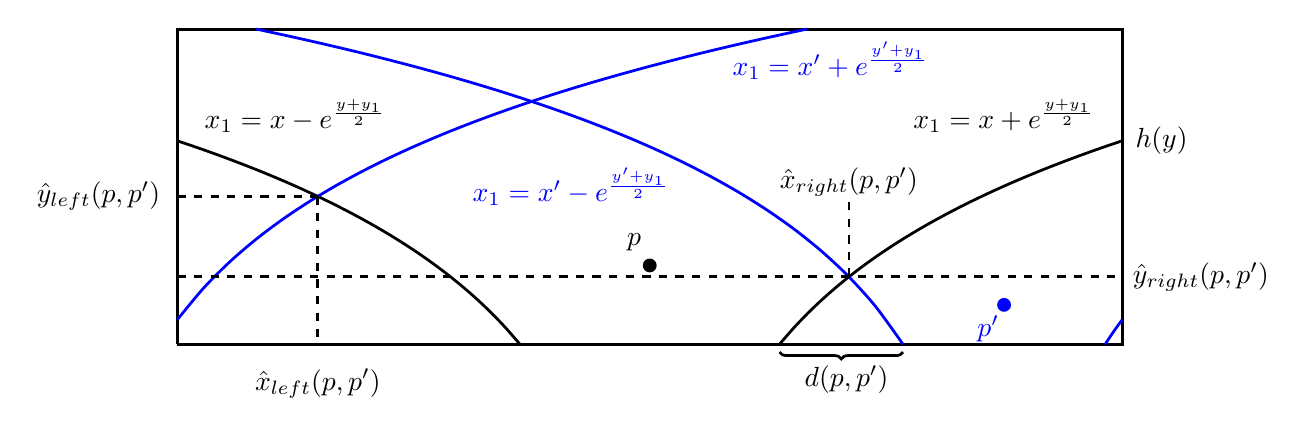
\begin{tikzpicture}
	

	\pgfmathsetmacro{\u}{0} %0
	\pgfmathsetmacro{\v}{1} %1
	\pgfmathsetmacro{\uu}{4.5} %1.4
	\pgfmathsetmacro{\vv}{0.5} %0.8
	\pgfmathsetmacro{\r}{6}
	\pgfmathsetmacro{\t}{4}
	
	%The box \Rcal
	\draw[line width=1pt] (-\r,0) -- (\r,0) -- (\r,\t) -- (-\r,\t) -- (-\r,0);
	
    \draw node[fill, circle, inner sep=0pt, minimum size=5pt] at (\u,\v) {};
    \draw node at (-0.2,1.3) {$p$};
    
    \draw node[fill,blue, circle, inner sep=0pt, minimum size=5pt] at (\uu,\vv) {};
    \draw node at (4.3,0.2) {\color{blue}$p^\prime$};
	
	\draw[domain=1.6487:6,smooth,variable=\x,black,line width=1pt] plot (\x, {2*ln(\x)-1});
    \draw[domain=-1.6487:-6,smooth,variable=\x,black,line width=1pt] plot (\x, {2*ln(-\x)-1});
    \draw[domain=5.7840:6,smooth,variable=\x,blue,line width=1pt] plot (\x, {2*ln(\x-4.5)-0.5});
    \draw[domain=3.2160:-5,smooth,variable=\x,blue,line width=1pt] plot (\x, {2*ln(4.5-\x)-0.5});
    \draw[domain=2:-6,smooth,variable=\x,blue,line width=1pt] plot (\x, {2*ln(\x+7.5)-0.5});
    
    
    
    \draw [decorate,decoration={brace},line width=1pt] (3.2160,-0.1) -- (1.6487,-0.1);
    \draw node at (2.5,-0.45) {$d(p,p^\prime)$};
    
%    \draw [dotted,line width=1pt] (2.5298,0.8563) -- (2.5298,1.7);
%    \draw node at (2.5298,2) {$\hat{x}(p,p^\prime)$};
    
    %Define intersection left black and shifted blue curve
    \pgfmathsetmacro{\vast}{2*ln((2*\r - \uu)/(exp(\v/2) + exp(\vv/2)))}
    \pgfmathsetmacro{\uast}{(\uu - 2*\r)/(1+exp((\vv-\v)/2))}
    %Define intersection right black and left blue curve
    \pgfmathsetmacro{\vvast}{2*ln((\uu)/(exp(\v/2) + exp(\vv/2)))}
    \pgfmathsetmacro{\uuast}{(\u*exp(\vv/2) + \uu*exp(\v/2))/(exp(\v/2) + exp(\vv/2))}
    \pgfmathsetmacro{\h}{2*ln(\r)-\v}
%    \draw[dotted,thick,black] (4.5208,2.0174) -- (4.5208,0);
%    \draw[dotted,thick,black] (4.5208,2.0174) -- (6,2.0174);
    
%    \draw node at (4.5208,-0.5) {$w_x(p,p^\prime)$};
%    \draw node at (7,2.0174) {$w_y(p,p^\prime)$};
    
    \draw node at (\r+0.5,\h) {$h(y)$};
    
    \draw node at (2.3,3.6) {\color{blue}$x_1 = x^\prime + e^{\frac{y^\prime + y_1}{2}}$};
    \draw node at (-1,2) {\color{blue}$x_1 = x^\prime - e^{\frac{y^\prime + y_1}{2}}$};
    \draw node at (-4.5,2.9) {$x_1 = x - e^{\frac{y + y_1}{2}}$};
    \draw node at (4.5,2.9) {$x_1 = x + e^{\frac{y + y_1}{2}}$};
	
	
	\draw[dashed,black,line width=1pt] (-\r,\vast) -- (\uast,\vast);
	\draw node at (-\r-1,\vast) {\color{black}$\hat{y}_{\text{left}}(p,p^\prime)$};
	\draw[dashed,line width=1pt] (\uast,\vast) -- (\uast,0);
	\draw node at (\uast,-0.5) {$\hat{x}_{\text{left}}(p,p^\prime)$};

	\draw[dashed,black,line width=1pt] (-\r,\vvast) -- (\r,\vvast);
	\draw node at (\r+1,\vvast) {\color{black}$\hat{y}_{\text{right}}(p,p^\prime)$};
	\draw[dashed,line width=1pt] (\uuast,\vvast) -- (\uuast,\vvast+1);
	\draw node at (\uuast,\vvast+1.2) {$\hat{x}_{\text{right}}(p,p^\prime)$};
	
	
\end{tikzpicture}
\caption{Schematic representation of the neighbourhoods of $p$ and $p^\prime$ in $\Gbox$ when $|x - x^\prime| > e^{\frac{y}{2}} + e^{\frac{y^\prime}{2}}$ used for the proof of Lemma \ref{lem:disjoint_neighbours_P_n_large}. Note that although here $p^\prime \notin \BallPon{p}$, this is not true in general. This situation was merely chosen to improve readability of the figure.}
\label{fig:representation_disjoint_neighbourhoods_P_n_3}
\end{figure}


We start by analyzing the shape of joint neighbourhood. Due to symmetry and the fact that we have identified the left and right boundaries of the box $\Rcal$, we can, without loss of generality, assume that $p = (0,y)$ and $p^\prime = (x^\prime,y^\prime)$ with $x^\prime > 0$. To understand the computation it is helpful to have a picture. Figure~\ref{fig:representation_disjoint_neighbourhoods_P_n_3} shows such an example. There are several different quantities that are important. The first are the heights where the left and right boundaries of the ball $\BallPon{p}$ go outside the box $\Rcal$. Since $x = 0$ these heights are the same and we denote this by $h(y)$. We also need to know the coordinates $\hat{y}_{\text{right}}(p,p^\prime)$ and $\hat{x}_{\text{right}}(p,p^\prime)$ of the intersection of the right boundary of the neighbourhood of $p$ with the left boundary of the neighbourhood of $p^\prime$ and those for the intersection of the left boundary of the neighbourhood of $p$ with the right boundary of the neighbourhood of $p^\prime$, which we denote by $\hat{y}_{\text{left}}(p,p^\prime)$ and $\hat{x}_{\text{left}}(p,p^\prime)$. Finally we will denote by $d(p,p^\prime)$ the distance between the lower right boundary of $\BallPon{p}$ and the lower left of $\BallPon{p^\prime}$, which is positive only when the bottom parts of both neighbourhoods do not intersect, as is the case in Figure~\ref{fig:representation_disjoint_neighbourhoods_P_n_3}. The condition $d(p,p^\prime) > 0$ is exactly the right notion for $p$ and $p^\prime$ being sufficiently separated.

Note that $\hat{y}_{\text{left}}(p,p^\prime)$ and $\hat{x}_{\text{left}}(p,p^\prime)$ correspond to, respectively, $\hat{y}(p,p^\prime)$ and $\hat{x}(p,p^\prime)$ considered in Section~\ref{ssec:missing_triangles}. The derivation of $\hat{y}_{\text{right}}(p,p^\prime)$ and $\hat{x}_{\text{right}}(p,p^\prime)$ is done in a similar manner and we omit the details here. The full expressions of all these functions are given below for further reference.

\begin{align}
	h(y) &= R_n - y + 2\log\left(\frac{\pi}{2}\right) \label{eq:def_height_y_P_n}\\
	h_1(p^\prime) &= 2\log\left(x^\prime + \frac{\pi}{2}e^{\frac{R_n}{2}}\right) - y^\prime \label{eq:def_height_left_P_n} \\
	h_2(p^\prime) &= 2\log\left(\frac{\pi}{2}e^{\frac{R_n}{2}} - x^\prime\right) - y^\prime 
		\label{eq:def_height_right_P_n} \\
%	\iota_x(p,p^\prime) &= \frac{(x^\prime-x)e^{\frac{y}{2}}}{e^{\frac{y}{2}} - e^{\frac{y^\prime}{2}}}
%		\label{eq:def_x_intersection_close_boundaries}\\
%	\iota_y(p,p^\prime) &= 2\log\left(\frac{x^\prime - x}{e^{\frac{y}{2}} - e^{\frac{y^\prime}{2}}}\right)
%		\label{eq:def_y_intersection_close_boundaries}\\
	\hat{y}_{\text{right}}(p,p^\prime) &= 2\log\left(\frac{x^\prime}{e^{\frac{y}{2}} + e^{\frac{y^\prime}{2}}}\right)\\
	\hat{x}_{\text{right}}(p,p^\prime) &= \frac{x^\prime}{1 + 	
		e^{\frac{y^\prime - y}{2}}},\\
	\hat{y}_{\text{left}}(p,p^\prime) &= 2 \log\left(\frac{\pi e^{R_n/2} - x^\prime}{e^{y/2} + e^{y^\prime/2}}\right),\\
	\hat{x}_{\text{left}}(p,p^\prime) &= \frac{x^\prime - \pi e^{R_n/2}}{1 + e^{\frac{y^\prime - y}{2}}}, \\
	d(p,p^\prime) &= |x - x^\prime| - \left(e^{\frac{y}{2}} + e^{\frac{y^\prime}{2}}\right).
	\label{eq:def_d_p_p_prime}
\end{align}

%We start with the result for points whose $x$-coordinates are close, which is when $d(p,p^\prime) < 0$.
%
%\begin{lemma}\label{lem:disjoint_neighbours_P_n}
%Let $p, p ^\prime \in \Rcal$ and denote $y^\ast = \min\{y, y^\prime\}$. Then whenever $|x - x^\prime| \le e^{\frac{y}{2}} + e^{\frac{y^\prime}{2}}$,
%\begin{align*}
%	\Exp{\Ncal_{\text{box}}(p \Delta p^\prime)}
%	&\ge \frac{\nu}{\pi}|x^\prime - x|\left(1 - \left(\frac{2}{\pi}\right)^{2\alpha}e^{-\alpha(R_n - y^\ast)}\right)\\
%	&\hspace{10pt}+ \xi\left|e^{\frac{y}{2}} - e^{\frac{y^\prime}{2}}\right|
%		\left(1 - \left(\frac{2}{\pi}\right)^{2\alpha - 1}e^{-(\alpha - \frac{1}{2})(R_n-y^\ast)}\right).
%\end{align*}
%\end{lemma}
%
%\begin{proof}
%In order to proof the result we will consider the area in between the two left boundaries of the balls $\BallPon{p}$ and
%$\BallPon{p^\prime}$ up to the height $h^\ast := \min\{h(y), h_2(p^\prime)\}$, see Figure~\ref{fig:representation_disjoint_neighbourhoods_P_n} and Figure~\ref{fig:representation_disjoint_neighbourhoods_P_n_2} for reference. Note that here we do not need to consider different cases depending on whether $|x - x^\prime| \le e^{(y + y^\prime)/2}$ or $|x - x^\prime| > e^{(y + y^\prime)/2}$. 
%
%By the Campbell-Mecke formula we get
%\begin{align*}
%	\Exp{\Ncal_{\text{box}}(p \Delta p^\prime)} &=	\Mu{\BallPon{p} \Delta B_{\Pcal,n}(p^\prime)}\\
%	&\ge \int_0^{h^\ast} \int_{x - e^{\frac{y + y_1}{2}}}^{x^\prime - e^{\frac{y^\prime + y_1}{2}}} f(x_1,y_1)
%		\, dx_1 \, dy_1 \\
%	&= \frac{\alpha \nu}{\pi}|x^\prime - x| \int_{0}^{h^\ast} e^{-\alpha y_1} dy_1
%		+ \frac{\alpha \nu}{\pi}\left|e^{\frac{y}{2}} - e^{\frac{y^\prime}{2}}\right| \int_0^{h^\ast} 
%		e^{-(\alpha-\frac{1}{2})y_1} \, dy_1\\
%	&= \frac{\nu}{\pi}|x^\prime - x|\left(1 - \left(\frac{2}{\pi}\right)^{2\alpha}e^{-\alpha(R_n - y^\ast)}\right)\\
%	&\hspace{10pt}+ \xi\left|e^{\frac{y}{2}} - e^{\frac{y^\prime}{2}}\right|
%		\left(1 - \left(\frac{2}{\pi}\right)^{2\alpha - 1}e^{-(\alpha - \frac{1}{2})(R_n-y^\ast)}\right).
%\end{align*}
%\end{proof}
%
%Now we will consider the case where $|x - x^\prime| > e^{\frac{y}{2}} + e^{\frac{y^\prime}{2}}$
%
%\begin{lemma}\label{lem:disjoint_neighbours_P_n_large}
%Let $p, p^\prime \in \Rcal$. Then, whenever $|x - x^\prime| > e^{\frac{y}{2}} + e^{\frac{y^\prime}{2}}$,
%\[
%	\Exp{\Ncal_{\text{box}}(p\Delta p^\prime)}
%	\ge \left(\mu(\BallPon{p}) + \mu(\BallPon{p^\prime})\right)
%		\left(1-\phi_n(p,p^\prime)\right).
%\]
%
%\[
%	\phi_n(p,p^\prime) = \xi\left( \left(\frac{e^{y/2} + e^{y^\prime/2}}{|x-x^\prime|}\right)^{2\alpha - 1}
%	- e^{-(\alpha - \frac{1}{2})R_n}\right)
%\]
%\end{lemma}
%
%\begin{proof}
%Without loss of generality we take $p = p_0 = (0,y)$ and $p^\prime = (x^\prime,y^\prime)$ with $0 \le x^\prime \le \frac{\pi}{2}e^{R/2}$. To state the result for general $p = (x,y)$ we use that $x^\prime = |x - x^\prime|$. In particular, we need to keep track of the minus sign in front of $x^\prime$. Note that for all $0 \le x^\prime \le \frac{\pi}{2}e^{R/2}$ it holds that $\hat{y}_{\text{right}}(p,p^\prime) \le \hat{y}_{\text{left}}(p,p^\prime)$ and hence
%\[
%	\Exp{\Ncal_{\text{box}}(p\Delta p^\prime)} 
%	\ge \int_0^{\hat{y}_{\text{right}}(p,p^\prime)} \int_{-\frac{\pi}{2}e^{\frac{R_n}{2}}}^{\frac{\pi}{2}e^{\frac{R_n}{2}}} \ind{p_1 \in \BallPon{p} \cup \BallPon{p^\prime}} f(x_1,y_1) \, dx_1 \, dy_1,
%\]
%We shall compute the integral on the right. We refer to Figure~\ref{fig:representation_disjoint_neighbourhoods_P_n_3} for further clarification. 
%
%Before we proceed we show that the neighbourhoods of $p$ and $p^\prime$ below $\hat{y}_{\text{right}}(p,p^\prime)$ are disjoint. This is clearly true when $\hat{y}_{\text{right}}(p,p^\prime) \le h_2(p^\prime)$ so suppose that $\hat{y}_{\text{right}}(p,p^\prime) > h_2(p^\prime)$. Then, because we identified the right and left boundaries of the box $\Rcal$ the right boundary of $\BallPon{p^\prime}$ continues from the left boundary of the box and is described by the equation
%\[
%	x_1 = x^\prime + e^{\frac{y^\prime + y_1}{2}} - \pi e^{\frac{R_n}{2}}.
%\]
%Now, let $x_{\mathrm{right}}^\prime$ and $x_{\mathrm{left}}$ denote the $x$-coordinate of the intersection of the line $\hat{y}_{\text{right}}(p,p^\prime)$ with, respectively, the right boundary of $\BallPon{p^\prime}$ and the left boundary of $\BallPon{p}$. Then, since $2x^\prime \le \pi e^{R/2}$,
%\begin{align*}
%	x_{\mathrm{right}}^\prime &= x^\prime + e^{\frac{y^\prime + \hat{y}_{\text{right}}(p,p^\prime)}{2}} - \pi e^{\frac{R_n}{2}}\\
%	&= x^\prime + e^{\frac{\hat{y}_{\text{right}}(p,p^\prime)}{2}}\left(e^{\frac{y}{2}} + e^{\frac{y^\prime}{2}}\right)
%		- e^{\frac{y + \hat{y}_{\text{right}}(p,p^\prime)}{2}} - \pi e^{\frac{R_n}{2}}\\
%	&= 2x^\prime - e^{\frac{y + \hat{y}_{\text{right}}(p,p^\prime)}{2}} - \pi e^{\frac{R_n}{2}}\\
%	&\le - e^{\frac{y + \hat{y}_{\text{right}}(p,p^\prime)}{2}} = x_{\mathrm{left}},
%\end{align*}
%and hence the neighbourhoods of $p$ and $p^\prime$ below $\hat{y}_{\text{right}}(p,p^\prime)$ are disjoint. It then follows that
%\begin{align*}
%	\Exp{\Ncal_{\text{box}}(p,p^\prime)} 
%	&\ge \int_0^{\hat{y}_{\text{right}}(p,p^\prime)} \int_{-\frac{\pi}{2}e^{\frac{R_n}{2}}}^{\frac{\pi}{2}e^{\frac{R_n}{2}}} 
%		\ind{p_1 \in \BallPon{p} \cup \BallPon{p^\prime}} f(x_1,y_1) \, dx_1 \, dy_1\\
%	&= \int_0^{\hat{y}_{\text{right}}(p,p^\prime)} \int_{-\frac{\pi}{2}e^{\frac{R_n}{2}}}^{\frac{\pi}{2}e^{\frac{R_n}{2}}} 
%		\left(\ind{p_1 \in \BallPon{p}} + \ind{p_1 \in \BallPon{p^\prime}}\right) 
%		f(x_1,y_1) \, dx_1 \, dy_1\\
%	&= \left(\mu_{\alpha,\nu ,n}(\BallPon{p}) + \mu_{\alpha,\nu ,n}(\BallPon{p^\prime})\right)
%		\left(1 - \frac{2\alpha \nu}{\pi}\int_{\hat{y}_{\text{right}}(p,p^\prime)}^{R_n} e^{-(\alpha - \frac{1}{2})y_1} \, dy_1\right),
%\end{align*}
%from which the result follows since
%\begin{align*}
%	\frac{2\alpha \nu}{\pi}\int_{\hat{y}_{\text{right}}(p,p^\prime)}^{R_n} e^{-(\alpha - \frac{1}{2})y_1} \, dy_1 
%	&= \xi\left(e^{-(\alpha - \frac{1}{2})\hat{y}_{\text{right}}(p,p^\prime)} - e^{-(\alpha - \frac{1}{2})R_n}\right)\\
%	&= \xi\left(\left(\frac{e^{y/2} + e^{y^\prime/2}}{x^\prime}\right)^{2\alpha - 1}
%		- e^{-(\alpha - \frac{1}{2})R_n}\right)\\
%	&= \xi\left(\left(\frac{e^{y/2} + e^{y^\prime/2}}{|x - x^\prime|}\right)^{2\alpha - 1}
%		- e^{-(\alpha - \frac{1}{2})R_n}\right)
%\end{align*}
%\end{proof}

%\begin{figure}
%\centering
%\begin{tikzpicture}
%	
%	%The box \Rcal
%	\draw (-5,0) -- (10,0);
%	\draw (-5,4) -- (10,4);
%	
%	
%	\draw[domain=1:5,smooth,variable=\x,black] plot (\x, {2*ln(\x)});
%    \draw[domain=-1:-5,smooth,variable=\x,black] plot (\x, {2*ln(-\x)});
%    \draw[domain=6:10,smooth,variable=\x,black] plot (\x, {2*ln(\x-5)});
%    \draw[domain=0:4,smooth,variable=\x,black] plot (\x, {2*ln(5-\x)});
%    
%    
%    
%    \draw node at (-1,2.5) {$\BallPo{p} \setminus B_{\Pcal}(p^\prime)$};
%    
%    \draw node at (-0.2,3.6) {$x_1 = x^\prime - e^{\frac{y^\prime+y_1}{2}}$};
%    
%    \draw node at (2.5,3) {$\Ncal_{\Pcal}(p,p^\prime)$};
%    
%    \draw node at (5.2,3.6) {$x_2 = x+e^{\frac{y+y_2}{2}}$};
%    
%    \draw node at (6,2.5) {$B_{\Pcal}(p^\prime) \setminus \BallPo{p}$};
%    
%    \draw[dashed,thick] (2.5,1.8326) -- (2.5,0.7);
%    \draw node at (2.5,0.4) {$w(p,p^\prime)$};
%    
%    \draw[dashed,thick] (-3,1.8326) -- (8,1.8326);
%    \draw node at (-4,1.8326) {$h(p,p^\prime)$};
%    
%    \draw [decorate,decoration={brace},line width=1pt] (4,-0.1) -- (1,-0.1);
%    \draw node at (2.5,-0.45) {$d(p,p^\prime)$};
%    
%    \draw node[fill, circle, inner sep=0pt, minimum size=5pt] at (0,0) {};
%    \draw node at (0,-0.5) {$p$};
%    
%    \draw node[fill, circle, inner sep=0pt, minimum size=5pt] at (5,0) {};
%    \draw node at (5,-0.5) {$p^\prime$};
%\end{tikzpicture}
%\caption{Schematic representation of the neighbourhoods of $p$ and $p^\prime$ in $\Gbox$ used for the proof of Lemma \ref{lem:common_neighbours_Pcal_n}.}
%\label{fig:representation_joint_neighbourhoods}
%\end{figure}

The following result shows that if $d(p,p^\prime) > 0$, then the expected number of common neighbours is $\smallO{\Mu{\BallPon{p}} + \Mu{\BallPon{p^\prime}}}$.

\begin{lemma}\label{lem:common_neighbours_Pcal_n}
Let $p, p^\prime \in \Rcal$. Then, whenever $|x - x^\prime| > \left(e^{\frac{y}{2}} + e^{\frac{y^\prime}{2}}\right)$,
\[
	\Exp{\Ncal_{\text{box}}(p,p^\prime)} \le \left(\Mu{\BallPon{p}} + \Mu{\BallPon{p^\prime}}\right)\phi_n(p,p^\prime),
\]
where
\[
	\phi_n(p,p^\prime) = 2\left(\frac{|x - x^\prime|}{e^{\frac{y}{2}} + e^{\frac{y^\prime}{2}}}\right)^{-(2\alpha - 1)} 
	+ \frac{3 \nu^{2\alpha + 1}e^{-(\alpha - \frac{1}{2})R} e^{\alpha y}}{2 \pi^{2\alpha}\left(
	e^{\frac{y}{2}} + e^{\frac{y^\prime}{2}}\right)}
	+ \frac{\nu e^{-(\alpha - \frac{1}{2})R}}{e^{\frac{y}{2}} + e^{\frac{y^\prime}{2}}}. 
\]
\end{lemma}

\begin{proof}
Again, without loss of generality we assume that $p = p_0 = (0,y)$ and $p^\prime = (x^\prime, y^\prime)$ with $0 \le x^\prime \le \frac{\pi}{2} e^{R/2}$. Consider the following two areas
\begin{align*}
	A_1 &:= \left\{(x_1,y_1) \in \Rcal \, : \, y_1 \ge \hat{y}_{\text{left}}(p_0,p^\prime), \, 
		-\frac{\pi}{2} e^{R/2} \wedge - e^{\frac{y + y_1}{2}} \le x_1 \le x^\prime + e^{\frac{y^\prime + y_2}{2}} - \pi e^{R/2} \right\}\\
	A_2 &:= \left\{(x_1,y_1) \in \Rcal \, : \, y_1 \ge \hat{y}_{\text{right}}(p_0,p^\prime), \,
			x^\prime - e^{\frac{y^\prime + y_1}{2}} \le x_1 \le \frac{\pi}{2} e^{R/2} \vee e^{\frac{y + y_2}{2}} \right\}.
\end{align*}
That is $A_1$ and $A_2$ describe all point $p_1 \in \BallPon{p_0} \cap \BallPon{p}$ with, respectively, $y_1 \ge \hat{y}_{\text{left}}(p_0,p^\prime)$ and $y_1 \ge \hat{y}_{\text{right}}(p_0,p^\prime)$. It now follows that
\[
	\Exp{\Ncal_{\text{box}}(p,p^\prime)} \le \Mu{A_1} + \Mu{A_2},
\]
and we will proceed by computing the measures of both sets. 

For $A_1$ we have (see also Figure~\ref{fig:comparing_triangles_diff_intersections})
\begin{align*}
	\Mu{A_1} &= \int_{\hat{y}_{\text{left}}(p_0,p^\prime)}^{h(y)} 
		\int_{- e^{\frac{y + y_1}{2}}}^{x^\prime + e^{\frac{y^\prime+y_1}{2}} - \pi e^{R/2}} \hspace{-10pt} 
		f(x_1,y_1) \dd x_1 \dd y_1
		+ \int_{h(y)}^{R} \int_{-\frac{\pi}{2}e^{R/2}}^{x^\prime + e^{\frac{y^\prime+y_1}{2}} - \pi e^{R/2}} 
		\hspace{-10pt}  f(x_1,y_1) \dd x_1 \dd y_1.
\end{align*}
For the first integral we get
\begin{align*}
	&\hspace{-10pt}\int_{\hat{y}_{\text{left}}(p_0,p^\prime)}^{h(y)} 
		\int_{- e^{\frac{y + y_1}{2}}}^{x^\prime + e^{\frac{y^\prime+y_1}{2}} - \pi e^{R/2}} \hspace{-10pt} 
		f(x_1,y_1) \dd x_1 \dd y_1\\
	&= \frac{\alpha \nu}{\pi}\left(e^{\frac{y}{2}} + e^{\frac{y}{2}}\right) 	
		\int_{\hat{y}_{\text{left}}(p_0,p^\prime)}^{h(y)} e^{-(\alpha - \frac{1}{2})y_1} \dd y_1
		- \frac{\alpha \nu}{\pi}\left(\pi e^{R/2} - x^\prime \right) 
		\int_{\hat{y}_{\text{left}}(p_0,p^\prime)}^{h(y)} e^{-\alpha y_1} \dd y_1\\
	&= \xi \left(e^{\frac{y}{2}} + e^{\frac{y^\prime}{2}}\right)
		\left(e^{-(\alpha - \frac{1}{2})\hat{y}_{\text{left}}(p_0,p^\prime)}
		- e^{-(\alpha - \frac{1}{2})h(y)}\right)
		- \frac{\nu}{\pi} \left(\pi e^{R/2} - x^\prime\right)
		\left(e^{-\alpha\hat{y}_{\text{left}}(p_0,p^\prime)}
		- e^{-\alpha h(y)}\right).
%	&= \frac{2\alpha \nu}{\pi(2\alpha - 1)}\left(e^{\frac{y}{2}} + e^{\frac{y}{2}}\right)
%		\left(\left(\frac{\pi e^{R/2} - x^\prime}{e^{\frac{y}{2}} + e^{\frac{y^\prime}{2}}}\right)^{-(2\alpha - 1)}
%		- \left(\frac{\pi}{2}\right)^{-(2\alpha - 1)} e^{-(2\alpha - 1)(R-y)}\right)\\
%	&\hspace{10pt}- \frac{\nu}{\pi} \left(\pi e^{R/2} - x^\prime\right)
%		\left(\left(\frac{\pi e^{R/2} - x^\prime}{e^{\frac{y}{2}} + e^{\frac{y^\prime}{2}}}\right)^{-2\alpha}
%			- \left(\frac{\pi}{2}\right)^{-2\alpha} e^{-2\alpha(R-y)}\right)
\end{align*}
Similarly, the second integral equals
\begin{align*}
	&\hspace{-20pt}\int_{h(y)}^{R} \int_{-\frac{\pi}{2}e^{R/2}}^{x^\prime + e^{\frac{y^\prime+y_1}{2}} - \pi e^{R/2}} 
		\hspace{-10pt}  f(x_1,y_1) \dd x_1 \dd y_1\\
	&= \xi e^{\frac{y^\prime}{2}}\left(e^{-(\alpha - \frac{1}{2})h(y)} - e^{-(\alpha - \frac{1}{2})R}\right)
		- \frac{\nu}{\pi}\left(\pi e^{R/2} - x^\prime\right)
		\left(e^{-\alpha h(y)}- e^{-\alpha R}\right).
\end{align*}
Combining these results yields
\begin{align*}
	\Mu{A_1} &= \xi \left(e^{\frac{y}{2}} + e^{\frac{y^\prime}{2}}\right)
		e^{-(\alpha - \frac{1}{2})\hat{y}_{\text{left}}(p_0,p^\prime)}
		- \xi e^{\frac{y}{2}} e^{-(\alpha - \frac{1}{2})h(y)}
		- \xi e^{\frac{y^\prime}{2}} e^{-(\alpha-\frac{1}{2})R} \\
	&\hspace{10pt}- \frac{\nu}{\pi} \left(\pi e^{R/2} - x^\prime\right)
		e^{-\alpha\hat{y}_{\text{left}}(p_0,p^\prime)}
		+ \nu e^{R/2}e^{-\alpha h(y)} + \frac{\nu}{\pi}\left(\pi e^{R/2} - x^\prime\right) e^{-\alpha R}\\
	&\le \xi \left(e^{\frac{y}{2}} + e^{\frac{y^\prime}{2}}\right)
		e^{-(\alpha - \frac{1}{2})\hat{y}_{\text{left}}(p_0,p^\prime)}
		+ \nu e^{R/2}e^{-\alpha h(y)} + \nu e^{-(\alpha - \frac{1}{2}) R}.
\end{align*}

We now proceed with $A_2$. Here we have
\begin{align*}
	\Mu{A_2} &= \int_{\hat{y}_{\text{right}}(p_0,p^\prime)}^{h(y)} 
		\int_{x^\prime - e^{\frac{y^\prime + y_1}{2}}}^{e^{\frac{y+y_1}{2}}} \hspace{-2pt} 
		f(x_1,y_1) \dd x_1 \dd y_1
		+ \int_{h(y)}^{R} \int_{x^\prime - e^{\frac{y^\prime + y_1}{2}}}^{\frac{\pi}{2}e^{R/2}} 
		\hspace{-2pt}  f(x_1,y_1) \dd x_1 \dd y_1.
\end{align*}
Computing each integral separately we get
\begin{align*}
	&\hspace{-20pt}\int_{\hat{y}_{\text{right}}(p_0,p^\prime)}^{h(y)} 
		\int_{x^\prime - e^{\frac{y^\prime + y_1}{2}}}^{e^{\frac{y+y_1}{2}}} \hspace{-2pt} 
		f(x_1,y_1) \dd x_1 \dd y_1\\
	&= \xi \left(e^{\frac{y}{2}} + e^{\frac{y^\prime}{2}}\right)
		\left(e^{-(\alpha - \frac{1}{2})\hat{y}_{\text{right}}(p_0,p^\prime)} 
		- e^{-(\alpha - \frac{1}{2})h(y)}\right) 
		- \frac{\nu}{\pi} x^\prime \left(e^{\alpha \hat{y}_{\text{right}}(p_0,p^\prime)}
		 - e^{-\alpha h(y)}\right), 
\end{align*}
and
\begin{align*}
	&\hspace{-20pt}\int_{h(y)}^{R} \int_{x^\prime - e^{\frac{y^\prime + y_1}{2}}}^{\frac{\pi}{2}e^{R/2}} 
		\hspace{-2pt}  f(x_1,y_1) \dd x_1 \dd y_1\\
	&= \xi e^{\frac{y^\prime}{2}}\left(e^{-(\alpha - \frac{1}{2})h(y)} - e^{-(\alpha - \frac{1}{2})R}\right)
		+ \frac{\nu}{\pi}\left(\frac{\pi}{2}e^{R/2} - x^\prime\right)\left(e^{-\alpha h(y)} - e^{-\alpha R}\right).
\end{align*}
Combining these results we get
\begin{align*}
	\Mu{A_2} &= \xi \left(e^{\frac{y}{2}} + e^{\frac{y^\prime}{2}}\right)
		e^{-(\alpha - \frac{1}{2})\hat{y}_{\text{right}}(p_0,p^\prime)} 
		- \xi e^{\frac{y}{2}}e^{-(\alpha - \frac{1}{2})h(y)} 
		- \xi e^{\frac{y^\prime}{2}}e^{-(\alpha - \frac{1}{2})R} \\
	&\hspace{10pt}- \frac{\nu}{\pi} x^\prime e^{-\alpha \hat{y}_{\text{right}}(p_0,p^\prime)}
		+ \frac{\nu}{2} e^{R/2} e^{-\alpha h(y)} - \frac{\nu}{\pi}\left(\frac{\pi}{2}e^{R/2} - x^\prime\right)
		e^{-\alpha R}\\
	&\le \xi \left(e^{\frac{y}{2}} + e^{\frac{y^\prime}{2}}\right)
		e^{-(\alpha - \frac{1}{2})\hat{y}_{\text{right}}(p_0,p^\prime)} + \frac{\nu}{2} e^{R/2} e^{-\alpha h(y)}.
\end{align*}

Finally, by adding the results for $\Mu{A_1}$ and $\Mu{A_2}$ and using that $\xi e^{\frac{y}{2}} = \Mu{\BallPon{p_0}}$ and 
$\xi e^{\frac{y^\prime}{2}} = \Mu{\BallPon{p^\prime}}$, we get
\begin{align*}
	\Exp{\Ncal_{\text{box}}(p,p^\prime)} 
	&\le \left(\Mu{\BallPon{p_0}} + \Mu{\BallPon{p_0}} \right)
		\left(e^{-(\alpha - \frac{1}{2})\hat{y}_{\text{left}}(p_0,p^\prime)}
		+ e^{-(\alpha - \frac{1}{2})\hat{y}_{\text{right}}(p_0,p^\prime)} \right) \\
	&\hspace{10pt}+ \frac{3\nu}{2}e^{R/2} e^{-\alpha h(y)}
		+ \nu e^{-(\alpha -\frac{1}{2}) R}.
\end{align*}
Finally we recall that $\hat{y}_{\text{left}}(p_0,p^\prime) \ge \hat{y}_{\text{right}}(p_0,p^\prime)$ for all $0 \le x^\prime \le \frac{\pi}{2}e^{R/2}$ and that $h(y) = R - y + 2\log(\pi/\nu)$. Hence
\begin{align*}
	&\Exp{\Ncal_{\text{box}}(p,p^\prime)} \\
	&\le \left(\Mu{\BallPon{p_0}} + \Mu{\BallPon{p_0}} \right) 
		\left(2e^{-(\alpha - \frac{1}{2})\hat{y}_{\text{right}}(p_0,p^\prime)} +    
		\frac{3 \nu^{2\alpha + 1}e^{-(\alpha - \frac{1}{2})R} e^{\alpha y}}{2 \pi^{2\alpha}\left(
		e^{\frac{y}{2}} + e^{\frac{y^\prime}{2}}\right)}
		+ \frac{\nu e^{-(\alpha - \frac{1}{2})R}}{e^{\frac{y}{2}} + e^{\frac{y^\prime}{2}}}
		\right)
\end{align*}
and the result follows by plugging in 
\[
	\hat{y}_{\text{right}}(p_0,p^\prime) = 2 \log\left(\frac{x^\prime}{e^{\frac{y}{2}} + e^{\frac{y^\prime}{2}}}\right),
\]
and noting that $x^\prime$ is the same as $|x - x^\prime|$, by our generalization step.

\end{proof} 

\subsubsection*{Degrees}

We now return to the joint degree distribution of nodes in $\Gbox$. Recall the definition of $\mathcal{E}_\varepsilon(k_n)$
\[
	\mathcal{E}_{\varepsilon}(k_n) = \left\{(p,p^\prime) \in \Rcal \times \Rcal
			\, : \, y,y^\prime \in \Kcal_{C}(k_n) \text{ and } |x - x^\prime| > k_n^{1 + \varepsilon} \right\}. 
\]
The following result, which follows from Lemma~\ref{lem:common_neighbours_Pcal_n}, shows that on this set, the expected number of common neighbours is $\smallO{k_n}$.

\begin{lemma}\label{cor:expected_common_neighbours_Ecal_set}
Fix $0 < \varepsilon < 1$ and let $\varepsilon^\prime = \min\{\varepsilon(2\alpha - 1),\varepsilon\}$. Then for all $(p,p^\prime) \in \mathcal{E}_\varepsilon(k_n)$, as $n \to \infty$,
\[
	\Mu{\BallPon{p} \cup \BallPon{p^\prime}} = \bigO{k_n^{1-\varepsilon^\prime}}.
\] 
\end{lemma}

\begin{proof}
Since for all $(p,p^\prime) \in \mathcal{E}_\varepsilon(k_n)$ we have $\Mu{\BallPon{p}}, \Mu{\BallPon{p^\prime}} = \bigT{k_n}$, Lemma~\ref{lem:common_neighbours_Pcal_n} implies that
\[
	\Mu{\BallPon{p} \cup \BallPon{p^\prime}} \le \bigO{k_n} \phi_n(p,p^\prime),
\]
where
\[
	\phi_n(p,p^\prime) = 2\left(\frac{|x - x^\prime|}{e^{\frac{y}{2}} + e^{\frac{y^\prime}{2}}}\right)^{-(2\alpha - 1)} 
		+ \frac{3 \nu^{2\alpha + 1}e^{-(\alpha - \frac{1}{2})R} e^{\alpha y}}{2 \pi^{2\alpha}\left(
		e^{\frac{y}{2}} + e^{\frac{y^\prime}{2}}\right)}
		+ \frac{\nu e^{-(\alpha - \frac{1}{2})R}}{e^{\frac{y}{2}} + e^{\frac{y^\prime}{2}}}. 
\]
We thus need to show that $\phi_n(p,p^\prime) = \bigO{k_n^{-\varepsilon}}$. For $(p,p^\prime) \in \mathcal{E}_\varepsilon(k_n)$, it holds that $e^{y/2}, e^{y^\prime/2} = \bigT{k_n}$ and $|x - x^\prime| > k_n^{1+\varepsilon}$ and hence
\begin{align*}
	 2\left(\frac{|x - x^\prime|}{e^{\frac{y}{2}} + e^{\frac{y^\prime}{2}}}\right)^{-(2\alpha - 1)}
	 =	\bigO{k_n^{-\varepsilon(2\alpha - 1)}}
\end{align*}
For the second term in $\phi_n(p,p^\prime)$ we use that $e^{\alpha y^\ast} = \bigT{k_n^{2\alpha}}$ and $e^{R} = \bigT{n^2}$ to obtain
\[
	\frac{3 \nu^{2\alpha + 1}e^{-(\alpha - \frac{1}{2})R} e^{\alpha y}}{2 \pi^{2\alpha}\left(
			e^{\frac{y}{2}} + e^{\frac{y^\prime}{2}}\right)}
	= \bigO{1} n^{-(2\alpha - 1)} k_n^{2\alpha - 1} = \bigO{n^{-(\alpha - \frac{1}{2})}}.
\]
Finally, the third term satisfies $\bigO{n^{-(2\alpha - 1)}k_n^{-1}}$, and we conclude that
\[
	\phi_n(p,p^\prime) = \bigO{k_n^{-\varepsilon(2\alpha - 1)} + n^{-(\alpha - \frac{1}{2})}
	+ n^{-(2\alpha - 1)}k_n^{-1}} = \bigO{k_n^{-\varepsilon^\prime}},
\]
where we used that $\varepsilon^\prime = \min\{\varepsilon(2\alpha - 1),\varepsilon\}$. 
\end{proof}

As a corollary we get that on the set $\mathcal{E}_\varepsilon(k_n)$ the joint degree distribution in $\Gbox$ is asymptotically equivalent to the product of the degree distributions. We shall however prove a slightly stronger result (Lemma~\ref{lem:joint_degree_factorization}) which also takes care of bounded shifts $\rho_{\text{box}}(p,p^\prime,k_n - t,k_n - t^\prime)$, for some uniformly bounded $t, t^\prime \in \mathbb{Z}$. For this we first need the following simple result for Poisson distributions.

\begin{lemma}\label{lem:finite_shifts_poisson}
Let $k_n \to \infty$ be a sequence of integers and $X = \Po(\lambda_n)$ be a Poisson random variable with mean $\lambda_n$ satisfying
\[
		k_n - C\sqrt{k_n \log(k_n)} \le \lambda_n \le k_n + C\sqrt{k_n \log(k_n)}
\]
for some $C > 0$. Then, for any $t_n, s_n = O(1)$, as $n \to \infty$,
\[
	\Prob{X = k_n - t_n} \sim \Prob{X = k_n - s_n}.
\]
\end{lemma}

\begin{proof}
Note that $k_n > t_n, s_n$ for large enough $n$. Hence, using Stirling's formula, as $n \to \infty$,
\begin{align*}
	\frac{\Prob{X = k_n - t_n}}{\Prob{X = k_n - s_n}}
	&= \frac{(k_n - t_n - (s_n-t_n))!}{(k_n - t_n)!} \lambda_n^{s_n - t_n} \\
	&\sim \sqrt{\frac{k_n - s_n}{k_n - t_n}} \, \frac{(k_n-s_n)^{k_n - s_n}}{(k_n - t_n)^{k_n - t_n}} \, e^{t_n - s_n} 
		\lambda_n^{s_n-t_n} \\
	&= \sqrt{\ell_n} (\ell_n)^{k_n - t_n} e^{t_n - s_n} (k_n - s_n)^{t_n - s_n} \lambda_n^{s_n-t_n}\\
	&= \sqrt{\ell_n} e^{(k_n - t_n)\log(\ell_n) + t_n - s_n} \left(\frac{k_n - s_n}{\lambda_n}\right)^{s_n - t_n}
\end{align*}
where we wrote $\ell_n = (k_n - s_n)/(k_n - t_n)$. Note that $\ell_n \to 1$ and hence $\sqrt{\ell_n} \to 1$. Moreover, since $(k_n - s_n)/\lambda_n \to 1$ and $|s_n - t_n| = \bigO{1}$ we have that $\left(\frac{k_n - s_n}{\lambda_n}\right)^{s_n - t_n} \sim 1$ Therefore it remains to show that
\[
	\lim_{n \to \infty} e^{(k_n - t_n)\log(\ell_n) + t_n - s_n} = 1.
\] 
For this we note that for any $x$, such that $|x| \le 1/2$, we have 
\[
	x - x^2 \le \log(1+x) \le x.
\]
Write $x_n = \ell_n - 1 = \frac{t_n - s_n}{k_n - t_n}$. Then by the assumptions of the lemma, $x_n \to 0$, and thus, for $n$ large enough,
\[
	t_n - s_n - \frac{(t_n - s_n)^2}{k_n - t_n}
	\le (k_n-t)\log\left(\ell_n\right)
	\le t_n - s_n.
\]
In particular
\[
	e^{-\frac{(t_n-s_n)^2}{k_n-t_n}}
	\le e^{(k_n - t_n)\log(\ell_n) + t_n - s_n} \le 1,
\]
and the result follows since $\frac{(t_n-s_n)^2}{k_n-t_n} \to 0$.
\end{proof}

We can now prove the main result of this section.

\begin{lemma}\label{lem:joint_degree_factorization}
Let $0 < \varepsilon < 1$, $k_n \to \infty$ and let $t_n,t^\prime_n, s_n, s_n^\prime \in \mathbb{Z}$ be uniformly bounded.
Then for any $(p,p^\prime) \in \mathcal{E}_\varepsilon(k_n)$, as $n \to \infty$,
\begin{align*}
	\rho_{\text{box}}(p,p^\prime,k_n - t_n,k_n - t_n^\prime)
	&= (1+\smallO{1})\rho_{\text{box}}(p,k_n - s_n)\rho_{\text{box}}(p^\prime,k_n-s_n^\prime).
\end{align*}
\end{lemma}

\begin{proof}
Define the random variables
\begin{align*}
	X_1(p,p^\prime) &:= \Po\left(\Mu{\BallPon{p}\setminus \BallPon{p^\prime}}\right),\\
	X_2(p,p^\prime) &:= \Po\left(\Mu{\BallPon{p^\prime}\setminus \BallPon{p}}\right),\\
	Y(p,p^\prime) &:= \Po\left(\Mu{\BallPon{p} \cup \BallPon{p^\prime}}\right),
\end{align*}
so that
\begin{align*}
	\rho_{\text{box}}(p,p^\prime,k_n-t_n,k_n-t_n^\prime) &= \Prob{X_1(p,p^\prime) + Y(p,p^\prime) = k_n-t_n, X_2(p,p^\prime) + Y(p,p^\prime) = k_n - t_n^\prime}.
\end{align*}
Since by Lemma~\ref{cor:expected_common_neighbours_Ecal_set} $\Mu{\BallPon{p} \cup \BallPon{p^\prime}} = \bigO{k_n^{1-\varepsilon^\prime}}$, it follows from Lemma~\ref{lem:near_independence_poisson} that
\[
	\rho_{\text{box}}(p,p^\prime,k_n-t_n,k_n-t_n^\prime) = (1+\smallO{1})\rho_{\text{box}}(p,k_n-t_n)\rho_{\text{box}}(p^\prime,k_n-t_n^\prime).
\]
The result then follows by applying Lemma~\ref{lem:finite_shifts_poisson} twice.
\end{proof}

\subsection{Concentration result for main triangle contribution}\label{ssec:concentration_tilde_T}

We now turn to Proposition \ref{prop:concentration_tilde_T_P_n}. Before we dive into the proof let us first give a high level overview of the strategy and the flow of the arguments. 

Recall (see \eqref{eq:def_degree_triangle_count_in_K}) that for any $C > 0$
\[
	\widetilde{T}_{\text{box}}(k_n,C) = \sum_{p \in \Pcal_n \cap \Kcal_{C,n}(k_n)} \ind{\text{deg}_{\text{box}}(p) = k} \widetilde{T}_{\text{box}}(p)
\]
Then we have
\[
	\widetilde{T}_{\text{box}}(k_n,C)^2 = \hspace{-5pt} \sum_{p, p^\prime \in \Pcal_n \cap \Kcal_C(k_n)}
		\hspace{-3pt} \ind{\Dbox(p), \, \Dbox(p^\prime) = k_n} 
		\sum_{(p_1, p_2), (p_1^\prime, p_2^\prime) \in \Pcal_n}^{\ne} \hspace{-3pt}
		\widetilde{T}_{\Pcal}(p,p_1,p_2) \widetilde{T}_{\Pcal}(p^\prime, p_1^\prime, p_2^\prime),
\]
This expression can be written as the sums of several terms, depending on how $\{p, p_1, p_2\}$ and $\{p^\prime, p_1^\prime, p_2^\prime\}$ intersect. To this end we define, for $a \in \{0,1\}$ and $b \in \{0,1,2\}$,
\[
	I_{a,b} = \hspace{-3pt} \sum_{p, p^\prime \in \Pcal_n \cap \Kcal_C(k) \atop |\{p\} \cap \{p^\prime\}| = a}
	\hspace{-5pt} \ind{\Dbox(p), \, \Dbox(p^\prime) = k_n} J_b(p,p^\prime),
\]
where
\[
	J_b(p,p^\prime) = \hspace{-10pt} \sum_{p_1, p_2, p_1^\prime, p_2^\prime \in \Pcal_n 
		\atop |\{p_1, p_2\} \cap \{p_1^\prime, p_2^\prime\}| = b}^{\ne}
		\hspace{-5pt} T_{\Pcal,n}(p,p_1,p_2) T_{\Pcal,n}(p^\prime, p_1^\prime, p_2^\prime),
\]
with the summation being over all two distinct pairs $(p_1, p_2)$ and $(p_1^\prime, p_2^\prime)$. Then we have
\[
	\widetilde{T}_{\text{box}}(k, C)^2 = \sum_{a = 0}^1 \sum_{b = 0}^2 I_{a,b}.
\]

To prove Proposition \ref{prop:concentration_tilde_T_P_n} we will deal with each of the $I_{a,b}$ separately, showing that 
\begin{equation}\label{eq:variance_T_I_00}
	\Exp{I_{0,0}} = (1+\smallO{1})\Exp{\widetilde{T}_{\text{box}}(k_n,C)}^2
\end{equation}
and for all other combinations
\begin{equation}\label{eq:variance_T_I_ab}
	\Exp{I_{a,b}} = \smallO{\Exp{\widetilde{T}_{\text{box}}(k_n,C)}^2}.
\end{equation}
Note $I_{1,2} = \widetilde{T}_{\text{box}}(k_n,C)$ and since~\eqref{eq:scaling_exected_tilde_T} implies that $\Exp{\widetilde{T}_{\text{box}}(k_n,C)} \to \infty$, it follows that \eqref{eq:variance_T_I_ab} holds for $I_{1,2}$. 

Recall that $\Rcal(k_n,C) = [-I_n,I_n] \times \Kcal_{C}(k_n)$ and~\eqref{eq:def_joint_degree_set_E_growing_k}
\[
	\mathcal{E}_{\varepsilon}(k_n) = \left\{(p,p^\prime) \in \Rcal \times \Rcal
			\, : \, y,y^\prime \in \Kcal_{C}(k_n) \text{ and } |x - x^\prime| > k_n^{1 + \varepsilon} \right\}.
\]
Let $\mathcal{E}_\varepsilon(k_n)^c$ the same set but with $|x - x^\prime| \le k_n^{1 + \varepsilon}$ and denote by $I_{a,b}^\ast$ the the part of $I_{a,b}$ where $(p,p^\prime) \in \mathcal{E}_\varepsilon(k_n)$. Will split the analysis between $I_{a,b}^\ast$ and $I_{a,b} - I_{a,b}^\ast$. The idea for these two cases is that by Lemma~\ref{lem:joint_degree_factorization} it follows that on the set $\mathcal{E}_\varepsilon(k_n)$ and for any uniformly bounded $t, t^\prime \in \mathbb{Z}$, the joint degree distribution factorizes,
\[
	\rho_{\text{box}}(p,p^\prime,k_n + t,k_n+t^\prime) = (1 + \smallO{1})\rho_{\text{box}}(p,k_n)\rho_{\text{box}}(p,k_n).
\]
In particular this allows us to prove that $\Exp{I_{0,0}^\ast} = (1+\smallO{1})\Exp{\widetilde{T}_{\text{box}}(k_n,C)}^2$. 
On the other hand, the expected number of points in $\mathcal{E}_\varepsilon(k_n)^c$ is $\bigO{k_n^{1+\varepsilon} k_n^{-2\alpha} \Exp{\Nbox(k_n)}} = \smallO{\Exp{\Nbox(k_n)}^2}$, where the latter is the expected number of points in $\Rcal(k_n,C) \times \Rcal(k_n,C)$. Hence we expect the contributions coming from $\mathcal{E}_\varepsilon(k_n)^c$ to be negligible.


% and~\eqref{eq:variance_T_I_ab} we have to consider the cases $k_n = \bigT{1}$ and $k_n \to \infty$ separately. However, each case follows a similar strategy. First we define a set $\mathcal{E} \subseteq \Kcal_{C}(k_n) \times \Kcal_{C}(k_n)$ such that outside this set the contributions of $\Exp{I_{a,b}}$ are negligible while on this set the joint degree distribution factorizes. These will be the sets defined by~\eqref{eq:def_joint_degree_set_E_constant_k} and~\eqref{eq:def_joint_degree_set_E_growing_k}. In particular, for these sets we have that $a = 1$ is not possible and hence we only need to consider the three different cases for $b$. For $a =0 = b$, the factorization of the degree distributions will enable us to prove~\eqref{eq:transition_clustering_main_term}. For $b = 1, 2$ we derive sufficient bounds for $\Exp{J_b(p,p^\prime)}$ in terms of $k_n$ for $(p,p^\prime)$ in the set $\mathcal{E}$.

\begin{proof}[Proof of Proposition \ref{prop:concentration_tilde_T_P_n}]

Throughout this proof we set $i = |\{p^\prime, p_1, p_2, p_1^\prime, p_2^\prime\} \cap \BallPon{p}|$, $j = |\{p^\prime\} \cap \BallPon{p}|$ and define $i^\prime, j^\prime$ in a similar way by interchanging the primed and non-primed variables. In addition, we write $D_{\text{box}}(p,p^\prime,k,\ell)$ to denote the indicator that $|\BallPon{p} \cap (\Pcal_n \setminus \{p, p^\prime, p_1, p_2, p_1^\prime, p_2^\prime\})| = k$ and $|\BallPon{p^\prime} \cap (\Pcal_n \setminus \{p, p^\prime, p_1, p_2, p_1^\prime, p_2^\prime\})| = \ell$. Then, by the Campbell-Mecke formula
\begin{align*}
	&\Exp{\ind{\Dbox(p) = k_n, \Dbox(p^\prime) = k_n} J_b(p,p^\prime)}\\
	&= \Exp{\sum_{p_1, p_2, p_1^\prime, p_2^\prime \in \Pcal_n 
		\atop |\{p_1, p_2\} \cap \{p_1^\prime, p_2^\prime\}| = b}^{\ne}
			\hspace{-7pt} D_{\text{box}}(p,p^\prime, k_n-i,k_n- i^\prime) \,
			\widetilde{T}_{\text{box}}(p,p_1,p_2) \widetilde{T}_{\text{box}}(p^\prime, p_1^\prime, p_2^\prime)}
\end{align*}
where the sum is over all distinct pairs $(p_1, p_2)$ and $(p_1^\prime, p_2^\prime)$. We also that 
\[
	\Exp{T_\Pcal(k_n)} = \bigT{n k_n^{-(2\alpha - 1)} s_\alpha(k_n)}.
\]

We will now proceed to establish \eqref{eq:variance_T_I_00} and \eqref{eq:variance_T_I_ab}. 

\paragraph{Computing $\bm{I_{0,0}}$}
We first show that
\begin{equation}\label{eq:I_ab_ast_main}
	\Exp{I_{0,0} - I_{0,0}^\ast} = \smallO{\Exp{T_{\text{box}}(k_n,C)}^2},
\end{equation}
so that for the remainder of the proof we only need to consider $p, p^\prime \in \mathcal{E}_\varepsilon(k_n)$ and hence, we can apply Lemma \ref{lem:joint_degree_factorization}. 

%For this we note that by Lemma \ref{lem:disjoint_neighbours_P_n} and Lemma \ref{lem:disjoint_neighbours_P_n_large} we have for $p,p^\prime \in \Kcal_{\varepsilon}(k_n)$ that $\Exp{\left|\Ncal_{\text{box}}(p\Delta p^\prime)\right|} \le k_n^{\varepsilon}$ implies that eventually and $|x-x^\prime| \le k_n^{1+\varepsilon}$. In particular $|x - x^\prime| \le k_n^{1+\varepsilon}$ for all $(p, p^\prime) \in \mathcal{E}_{\varepsilon}(k_n)^c$. Therefore, we have
For $J_0$ we have, using Lemma~\ref{lem:joint_degree_factorization}
\begin{align*}
	&\Exp{\ind{\Dbox(p) = k_n, \Dbox(p^\prime) = k_n} J_0(p,p^\prime)}\\
	&= \Exp{\sum_{p_1, p_2, p_1^\prime, p_2^\prime \in \Pcal \setminus p,p^\prime 
		\atop |\{p_1, p_2\} \cap \{p_1^\prime, p_2^\prime\}| = 0}^{\ne}
		\hspace{-7pt} D_{\text{box}}(p,p^\prime, k_n-i,k_n- i^\prime) \,
		\widetilde{T}_{\text{box}}(p,p_1,p_2) \widetilde{T}_{\text{box}}(p^\prime, p_1^\prime, p_2^\prime)}\\
	&= \Exp{D_{\text{box}}(p,p^\prime, k_n-j-2,k_n- j^\prime-2) \, \sum_{p_1,p_2 \in \Pcal \setminus p}^{\ne} 
		\widetilde{T}_{\text{box}}(p,p_1,p_2)
		\sum_{p_1^\prime,p_2^\prime \in \Pcal \setminus p^\prime}^{\ne} 
			\widetilde{T}_{\text{box}}(p^\prime,p_1^\prime,p_2^\prime)}\\
	&= (1+\smallO{1})\rho_{\text{box}}(p,p^\prime,k_n,k_n) \CExp{\widetilde{T}_{\text{box}}(p)}{\Dbox(p) = k_n}
		\CExp{\widetilde{T}_{\text{box}}(p^\prime)}{\Dbox(p^\prime) = k_n},
\end{align*}
Next we recall that for all $y^\prime \in \Kcal_{C}(k_n)$, 
\[
	\CExp{\widetilde{T}_{\text{box}}(p^\prime)}{\Dbox(p^\prime) = k_n} = \binom{k_n}{2} \Mu{\BallPon{p^\prime}}^{-2} \Exp{\widetilde{T}_{\text{box}}(p^\prime)} = \bigO{1}k_n^2 P(y^\prime),
\] 
where we used that $\Exp{\widetilde{T}_{\text{box}}(p^\prime)} = (1+\smallO{1}) k_n^2 P(y^\prime)$, for all $y^\prime \in \Kcal_{C}(k_n)$. Therefore, using that $\rho_{\text{box}}(p,p^\prime,k_n,k_n) \le \rho_{\text{box}}(p,k_n)$,
\begin{align*}
	&\Exp{\ind{\Dbox(p) = k_n, \Dbox(p^\prime) = k_n} J_0(p,p^\prime)}\\
	&\le \bigO{k_n^2} \rho_{\text{box}}(p,k_n) \CExp{\widetilde{T}_{\text{box}}(p)}{\Dbox(p) = k_n} P(y^\prime)
\end{align*}
and thus
\begin{align*}
	&\Exp{I_{0,0} - I_{0,0}^\ast}\\
	&= \int_{\mathcal{E}_\varepsilon(k_n)^c}
		\Exp{\ind{\Dbox(p), \Dbox(p^\prime) = k_n} J_0(p,p^\prime)} f(x,y) f(x^\prime,y^\prime) \, dx^\prime \, dx \, dy^\prime \, dy\\
%	&= \int_{\Kcal_C(k_n)^2} \ind{|x-x^\prime| \le k_n^{1 + \varepsilon}}
%		\Exp{\ind{\Dbox(p), \Dbox(p^\prime) = k_n} J_0(p,p^\prime)} f(x,y) f(x^\prime,y^\prime) \, dx^\prime \, dx \, dy^\prime \, dy\\
	&\le \bigO{k_n^2} k_n^{1+\varepsilon} \left(\int_{a_n^-}^{a_n^+} P(y^\prime) 
		e^{-\alpha y^\prime} \, dy^\prime\right) \Exp{\widetilde{T}_{\text{box}}(k_n,C)}\\
	&= \bigO{k_n^{3 + \varepsilon -2\alpha} s_\alpha(k_n) \Exp{\widetilde{T}_{\text{box}}(k_n,C)}}\\
	&= \smallO{n k_n^{-(2\alpha - 1)}s_\alpha(k_n) \Exp{T_{\Pcal,n}(k_n)}} 
		= \smallO{\Exp{\widetilde{T}_{\text{box}}(k_n,C)}^2},
\end{align*}
which proves \eqref{eq:I_ab_ast_main}. Here we used that $k_n^{2 + \varepsilon} = \smallO{n}$ and
\[
	\Exp{\widetilde{T}_{\text{box}}(k_n,C)} = \bigT{\Exp{\widetilde{T}_{\text{box}}(k_n)}} 
	= \bigT{n k_n^{-(2\alpha - 1)}s_\alpha(k_n)}
\] 
for the last line.

We will now show that
\[
	\Exp{I^\ast_{0,0}} = (1+\smallO{1})\Exp{\Exp{T_{\text{box}}(k_n,C)}^2}.
\]
We recall that for $(p,p^\prime) \in \mathcal{E}_{\varepsilon}(k_n)$ and any two uniformly bounded $t, t^\prime \in \mathbb{Z}$,
\[
	\rho_{\text{box}}(p,p^\prime,k_n + t,k_n+t^\prime) = (1 + \smallO{1})\rho_{\text{box}}(p,k_n)\rho_{\text{box}}(p,k_n).
\]
Therefore, by defining $h(y) = \CExp{\widetilde{T}_{\text{box}}(y)}{\Dbox(y) = k_n}$
\[
	\Exp{I_{0,0}^\ast} = (1 + \smallO{1})\int_{\mathcal{E}_{\varepsilon}(k_n)}\rho_{\text{box}}(p,k_n)
		\rho_{\text{box}}(p^\prime,k_n)
		h(y) h(y^\prime) f(x,y)	f(x^\prime,y^\prime) \, dx^\prime \, dx \, dy^\prime \, dy.
\]
The difference with $\Exp{\Exp{T_{\text{box}}(k_n,C)}^2}$ is in that the above integral is over $\mathcal{E}_\varepsilon(k_n)$ instead of $\Rcal(k_n,C) \times \Rcal(k_n,C)$. Since the difference between the two sets is 
$\mathcal{E}_\varepsilon(k_n)^c$ and $n k_n^{1+\varepsilon} = \smallO{n^2}$ it follows that
\begin{align*}
	&\Exp{\Exp{T_{\text{box}}(k_n,C)}^2}
		- \int_{\mathcal{E}_{\varepsilon}(k_n)}\rho_{\text{box}}(p,k_n)\rho_{\text{box}}(p^\prime,k_n)
		h(y) h(y^\prime) f(x,y)	f(x^\prime,y^\prime) \dd x^\prime \dd x \dd y^\prime \dd y\\
	&= \int_{\mathcal{E}_{\varepsilon}(k_n)^c}\rho_{\text{box}}(p,k_n)\rho_{\text{box}}(p^\prime,k_n)
		h(y) h(y^\prime) f(x,y)	f(x^\prime,y^\prime) \dd x^\prime \dd x \dd y^\prime \dd y\\
	&= \bigO{k_n^{1+\varepsilon}n} 
		\left(\int_{\Kcal_{C}(k_n)}h(y)\rho_{\text{box}}(y,k_n)\alpha e^{-\alpha y} \dd y\right)^2
		= \smallO{\Exp{\Exp{T_{\text{box}}(k_n,C)}^2}}.
\end{align*}
Thus we conclude that $\Exp{I^\ast_{0,0}} = (1+\smallO{1})\Exp{\Exp{T_{\text{box}}(k_n,C)}^2}$, which finishes the proof of \eqref{eq:variance_T_I_00}.

\paragraph{Computing $\bm{\Exp{I_{0,1}}}$}

We first write
\begin{equation}\label{eq:bound_E_J1}
	\Exp{\ind{\Dbox(p) = k_n, \Dbox(p^\prime) = k_n} J_1}
	\le \bigO{1} k_n \rho_{\text{box}}(p,p^\prime,k_n,k_n)\CExp{\widetilde{T}_{\text{box}}(p)}{\Dbox{p} = k}
\end{equation}
Then, using that $\rho_{\text{box}}(p,p^\prime,k_n,k_n) \le \rho_{\text{box}}(p,k_n)$,
\begin{align*}
	&\Exp{I_{0,1} - I_{0,1}^\ast}\\
	&\int_{\mathcal{E}_\varepsilon(k_n)^c}
		\Exp{\ind{\Dbox(p), \Dbox(p^\prime) = k_n} J_1(p,p^\prime)} f(x,y) f(x^\prime,y^\prime) \, dx^\prime \, dx \, dy^\prime \, dy\\
	&= k_n \int_{\Kcal_C(k_n)^2} \ind{|x-x^\prime| \le k_n^{1 + \varepsilon}}
		\rho_{\text{box}}(p,k_n)\CExp{\widetilde{T}_{\text{box}}(p)}{\Dbox{p} = k} f(x,y) f(x^\prime,y^\prime) \, dx^\prime \, dx \, dy^\prime \, dy\\
	&\le \bigO{k_n^{2+\varepsilon}} \left(\int_{a_n^-}^{a_n^+} e^{-\alpha y^\prime} \, dy^\prime\right) 
		\Exp{\widetilde{T}_{\text{box}}(k_n,C)}\\
	&= \bigO{k_n^{2 + \varepsilon - 2\alpha} \Exp{\widetilde{T}_{\text{box}}(k_n,C)}}.
\end{align*}
Recall that $\Exp{\widetilde{T}_{\text{box}}(k_n,C)} = \bigT{n k_n^{-(2\alpha - 1)}s(k_n)}$. Therefore to show that $\Exp{I_{0,1} - I_{0,1}^\ast} = \smallO{\Exp{\widetilde{T}_{\text{box}}(k_n,C)}^2}$ it suffices to show that $k_n^{2 + \varepsilon - 2\alpha} = \smallO{n k_n^{-(2\alpha - 1)}s(k_n)}$. When $\frac{1}{2} < \alpha \le \frac{3}{4}$ we have
\[
	\frac{4\alpha - 1 + \varepsilon}{2\alpha + 1} < 1,
\]
for $\varepsilon$ small enough. Hence
\[
	n^{-1} k_n^{2\alpha - 1} s(k_n)^{-1} k_n^{2 + \varepsilon -2\alpha} = k_n^{4\alpha - 1 + \varepsilon} 
	= \smallO{n^{-1}n^{\frac{4\alpha - 1 + \varepsilon}{2\alpha + 1}}} = \smallO{1}
\]
When $\alpha \ge \frac{3}{4}$,
\[
	n^{-1} k_n^{2\alpha - 1} s(k_n)^{-1} k_n^{2 + \varepsilon -2\alpha} = \bigO{\log(k_n)} n^{-1} k_n^{2 + \varepsilon} = \smallO{1},
\]
for $\varepsilon$ small enough.

For $(p,p^\prime) \in \mathcal{E}_\varepsilon(k_n)$ we assume without loss of generality that $p_1^\prime = p_1 = (x_1,y_1)$, i.e.
\[
	J_{0,1} = \sum_{(p_1, p_2) \in \Pcal \setminus p}^{\ne} \widetilde{T}_{\text{box}}(p,p_1,p_2) 
	\sum_{p_2^\prime \in \Pcal \setminus \{p^\prime, p_1\}} \widetilde{T}_{\text{box}}(p^\prime,p_1,p_2^\prime). 
\] 
Now let $Z_{0,1}$ denote the part of $J_{0,1}$ where $y_1 \le 4\log(k_n)$ and $y_2, y_2^\prime \le \varepsilon \log(k_n)$. 

We first analyze $\CExp{Z_{0,1}}{\Dbox(p), \Dbox(p^\prime) = k_n}$. When $y_1 \le 4\log(k_n)$ and both $y_2, y_2^\prime \le \varepsilon \log(k_n)$ we have that
\[
	|x_2 - x_2^\prime| \le |x_1 - x_2| + |x_1 - x_2^\prime| \le e^{\frac{y_1}{2}}\left(e^{\frac{y_2}{2}} + e^{\frac{y_2^\prime}{2}}\right) \le 2k_n^{2+\varepsilon}
\]
whenever $\widetilde{T}_{\text{box}}(p,p_1,p_2) \widetilde{T}_{\text{box}}(p^\prime,p_1,p_2^\prime) > 0$ while both $|x - x_2|, |x^\prime - x_2^\prime| = \bigO{k_n^{1 + \varepsilon}}$. Hence it follows that $\widetilde{T}_{\text{box}}(p,p_1,p_2) \widetilde{T}_{\text{box}}(p^\prime,p_1,p_2^\prime) > 0$ implies that
\[
	|x - x^\prime| \le |x - x_2| + |x_2 - x_2^\prime| + |x_2^\prime - x^\prime| = \bigO{k_n^{2 + \varepsilon}}.
\]
Next, by integrating only over $x_2^\prime$ and $y_2^\prime $ we get that $\CExp{Z_{0,1}}{\Dbox(p), \Dbox(p^\prime) = k_n}$ 
\begin{align*}
	\CExp{Z_{0,1}}{\Dbox(p), \Dbox(p^\prime) = k_n} &=
	\bigO{e^{\frac{y^\prime}{2}}\ind{|x-x^\prime|\le k_n^{2 + \varepsilon}} 
		\CExp{\widetilde{T}_{\text{box}}(p)}{\Dbox(p) =k_n}}\\
	&= \bigO{k_n \CExp{\widetilde{T}_{\text{box}}(p)}{\Dbox(p) =k_n}}.
\end{align*}
Thus
\begin{align*}
	&\int_{\mathcal{E}_\varepsilon(k_n)} \rho_{\text{box}}(p,p^\prime,k_n,k_n)
		\CExp{Z_{0,1}}{\Dbox(p), \Dbox(p^\prime) = k_n} f(x,y) f(x^\prime,y^\prime) \dd x \dd y \dd x^\prime \dd y^\prime\\
	&= \bigO{k_n^{3+\varepsilon}} \Exp{\widetilde{T}_{\text{box}}(k_n,C)} 
		\int_{\Kcal_{C}(k_n)}\rho_{\text{box}}(y^\prime,k_n) e^{-\alpha y^\prime} \dd y^\prime\\
	&= \bigO{k_n^{2+\varepsilon} k_n^{-2\alpha} \Exp{\widetilde{T}_{\text{box}}(k_n,C)} } 
		= \smallO{\Exp{\widetilde{T}_{\text{box}}(k_n,C)}^2}, 
\end{align*}
where the last line follow from the analysis done for $\Exp{I_{0,0}-I_{0,0}^\ast}$.

It now remains to consider $J_{0,1} - Z_{0,1} := Z_{0,1}^\ast$. We will show that 
\begin{equation}\label{eq:expectation_J01}
	\CExp{Z_{0,1}^\ast}{\Dbox(p), \Dbox(p^\prime) = k_n} = \smallO{k_n^4 s(k_n)^2}.
\end{equation} 
Using that the joint degree distribution factorizes on $\mathcal{E}_\varepsilon(k_n)$ this then implies that
\begin{align*}
	\Exp{I_{0,1}^\ast}
%	&= \bigO{1} \int_{\mathcal{E}_\varepsilon(k_n)} \rho_{\text{box}}(p,k_n) \rho_{\text{box}}(p^\prime,k_n) \CExp{J_{0,1}}{\Dbox(p), \Dbox(p^\prime) = k_n} f(x,y) f(x^\prime,y^\prime) \, dx^\prime \, dx \, dy^\prime \, dy \\
	&= \smallO{k_n^4 s(k_n)^2} \left(\int_{\Rcal(k_n,C)} \rho_{\text{box}}(y,k_n) f(x,y) \dd x \dd y \right)^2\\ 
	&= \smallO{\left(n s(k_n) k_n^{-2\alpha + 1}\right)^2} = \smallO{\Exp{\widetilde{T}_{\text{box}}(k_n,C)}^2},
\end{align*}
which finished the proof of~\eqref{eq:variance_T_I_ab} for $a = 0, b = 1$.

We first consider the part with $y_1 > 4\log(k_n)$. Since the integration over $x_1, x_2$ and $x_2^\prime$ of $\CExp{Z_{0,1}^\ast}{\Dbox(p), \Dbox(p^\prime) = k_n}$ is bounded by $\bigO{e^{y}e^{\frac{y^\prime}{2}}}$ we get that the contribution to $\CExp{Z_{0,1}^\ast}{\Dbox(p), \Dbox(p^\prime) = k_n}$ with $y > 4\log(k_n)$ and $(p,p^\prime) \in \mathcal{E}_\varepsilon(k_n)$ is
\begin{align*}
	\bigO{e^{y}e^{\frac{y^\prime}{2}} \int_{4\log(k_n)}^{R} e^{-(\alpha - \frac{1}{2})y_1} \, dy_1}
	&= \bigO{k_n^3 \int_{4\log(k_n)}^{R} e^{-(\alpha - \frac{1}{2})y_1} \, dy_1}\\
	&= \bigO{k_n^{3 - (4\alpha - 2)}} = \smallO{k_n^4 s_\alpha(k_n)^2}.
\end{align*}
Here the last step follows since for $\frac{1}{2} < \alpha < \frac{3}{4}$
\[
	k_n^{3 - (4\alpha - 2) - 4} s(k_n)^{-2} 
	= k_n^{3 - (4\alpha - 2) - 4 + 2(4\alpha - 2)} = k_n^{-5 + 4\alpha} = \smallO{1},
\]
while for $\alpha = \frac{3}{4}$
\[
	k_n^{3 - (4\alpha - 2) - 4} s(k_n)^{-2} 
	= \bigO{\log(k_n)^{-2}} k_n^{3 - (4\alpha - 2) - 2} = \bigO{\log(k_n)^{-2}} = \smallO{1},
\]
and for $\alpha > \frac{3}{4}$
\[
	k_n^{3 - (4\alpha - 2) - 4} s(k_n)^{-2} = k_n^{3 - (4\alpha - 2) - 2} = \smallO{1}.
\]

Next we consider the case where $y_1 \le 4\log(k_n)$ and at least one of $y_2, y_2^\prime$ is larger than $\varepsilon \log(k_n)$. Due to symmetry it is enough to consider the case with $y_2 > \varepsilon \log(k_n)$. Here the contribution to $\CExp{Z_{0,1}^\ast}{\Dbox(p), \Dbox(p^\prime) = k_n}$ is
\begin{align*}
	\Exp{\widetilde{T}_{\text{box}}(p)}
		\bigO{e^{\frac{y^\prime}{2}}\int_{\varepsilon \log(k_n)}^{R} e^{-(\alpha -\frac{1}{2})y_2} \, dy_2}
	&= \bigO{k_n^{1 - \varepsilon(\alpha -\frac{1}{2})}}\Exp{\widetilde{T}_{\text{box}}(p)}\\
	&= \bigO{k_n^{3 - \varepsilon(\alpha -\frac{1}{2})} s(k_n)} = \smallO{k_n^4 s(k_n)^2}.
\end{align*}
The last line follows since $k_n^{-1} = \smallO{s(k_n)}$ for $\frac{1}{2} < \alpha < \frac{3}{4}$ and $k_n^{-1} = \bigO{s(k_n)}$ for $\alpha \ge \frac{3}{4}$. 

\paragraph{Computing $\bm{\Exp{I_{0,2}}}$} In this case we have
\[
	\Exp{\ind{\Dbox(p) = k_n, \Dbox(p^\prime) = k_n}J_2} = (1+\smallO{1})\rho_{\text{box}}(p,p^\prime,k_n,k_n)
	\CExp{\widetilde{T}_{\text{box}}(p)}{\Dbox(p) = k_n}.
\]
We then use that $\rho_{\text{box}}(p,p^\prime,k_n,k_n) \le \rho_{\text{box}}(p,k_n)$ to obtain
\begin{align*}
	\Exp{I_{0,2}-I_{0,2}^\ast} 
	&= \bigO{k_n^{1+\varepsilon}} \left(\int_{\Kcal_{C}(k_n)} e^{-\alpha y^\prime} \dd y^\prime\right) 
		\Exp{\widetilde{T}_{\text{box}}(k_n,C)}\\
	&= \bigO{k_n^{\varepsilon -(2\alpha - 1)}}\Exp{\widetilde{T}_{\text{box}}(k_n,C)}
		= \smallO{\Exp{\widetilde{T}_{\text{box}}(k_n,C)}}
\end{align*}
were the last line follows since $\Exp{\widetilde{T}_{\text{box}}(k_n,C)} = \bigT{n k_n^{-(2\alpha - 1)}s(k_n)}$ and $k_n^{\varepsilon}n^{-1} = \smallO{s(k_n)}$.

For the other term we use that the degree distribution factorizes. This gives
\begin{align*}
	\Exp{I_{0,2}^\ast} 
	&= \bigO{1}\left(\int_{\Rcal(k_n,C)} \rho_{\text{box}}(y^\prime,k_n) f(x^\prime,y^\prime) 
		\dd x^\prime \dd y^\prime \right)\Exp{\widetilde{T}_{\text{box}}(k_n,C)}\\
	&= \bigO{n k_n^{-(2\alpha + 1)}}\Exp{\widetilde{T}_{\text{box}}(k_n,C)}
		= \smallO{\Exp{\widetilde{T}_{\text{box}}(k_n,C)}^2},
\end{align*}
where we use that $k_n^{-2} = \smallO{s(k_n)}$.

\paragraph{Computing $\bm{\Exp{I_{1,1}}}$}

Using~\eqref{eq:expectation_J01} we get
\begin{align*}
	\Exp{I_{1,1}}
	&= \bigO{k_n} \int_{\Rcal(k_n,C)} \rho_{\text{box}}(y,k_n) \CExp{\widetilde{T}_{\text{box}}}{\Dbox(p) = k_n}
		f(x,y) \dd x \dd y\\
	&= \bigO{k_n}\Exp{\widetilde{T}_{\text{box}}(k_n,C)}.
\end{align*}
Now observe that for $\frac{1}{2} < \alpha < \frac{3}{4}$
\[
	k_n n^{-1} n^{-1} k_n^{-(2\alpha -1)} s(k_n)^{-1} = k_n^{6\alpha - 2} n^{-1}
	= \bigO{n^{\frac{4\alpha - 3}{2\alpha + 1}}} = \smallO{1},
\]
while for $\alpha \ge \frac{3}{4}$
\[
	k_n n^{-1} n^{-1} k_n^{-(2\alpha -1)} s(k_n)^{-1} = \bigO{n^{-1} k_n^{-(2\alpha - 1)}} = \smallO{1}.
\]
We conclude that $k_n = \smallO{n k^{-(2\alpha - 1)}s(k_n)}$ and hence $\Exp{I_{1,1}} = \smallO{\Exp{\widetilde{T}_{\text{box}}(k_n,C)}^2}$.


\end{proof}